% Chapter Template

\chapter{Simulation and Results} % Main chapter title

\label{Chapter4}
In this section we will going over all the part of our app one by one simulating a user’s
workflow.\par\noindent

\section{Login and Signup}
The landing page is the
first page that the user will see when he/she opens the app. The landing page is shown in\par
\begin{figure}[h]
    \centering
    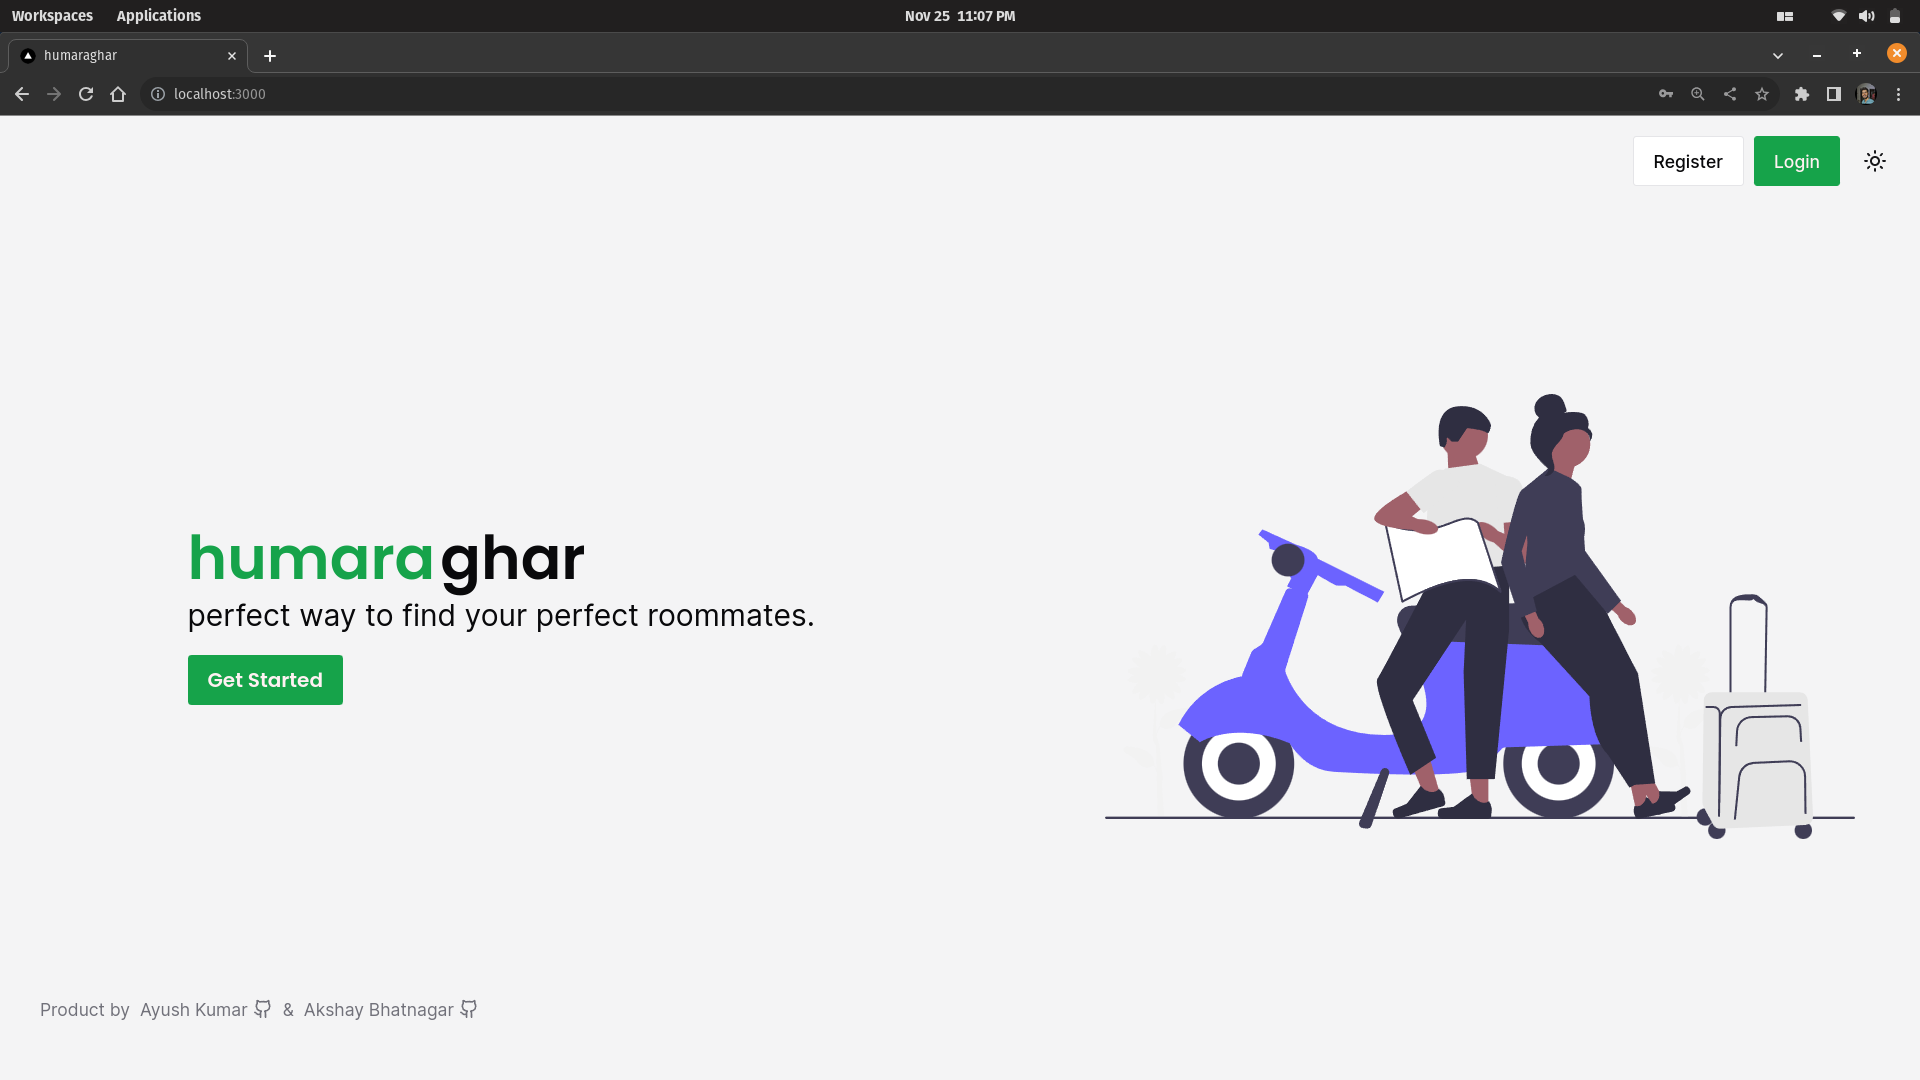
\includegraphics[width=1\textwidth]{Images/screenshots/landing.png}
    \caption{Landing Page}
\end{figure}
\noindent
The landing page contains a button that will take the user to the sign-up/login page or directly to the dashboard if
already signed in.\par\noindent

\clearpage
The sign-up/login page is shown in \par
\begin{figure}[h]
    \centering
    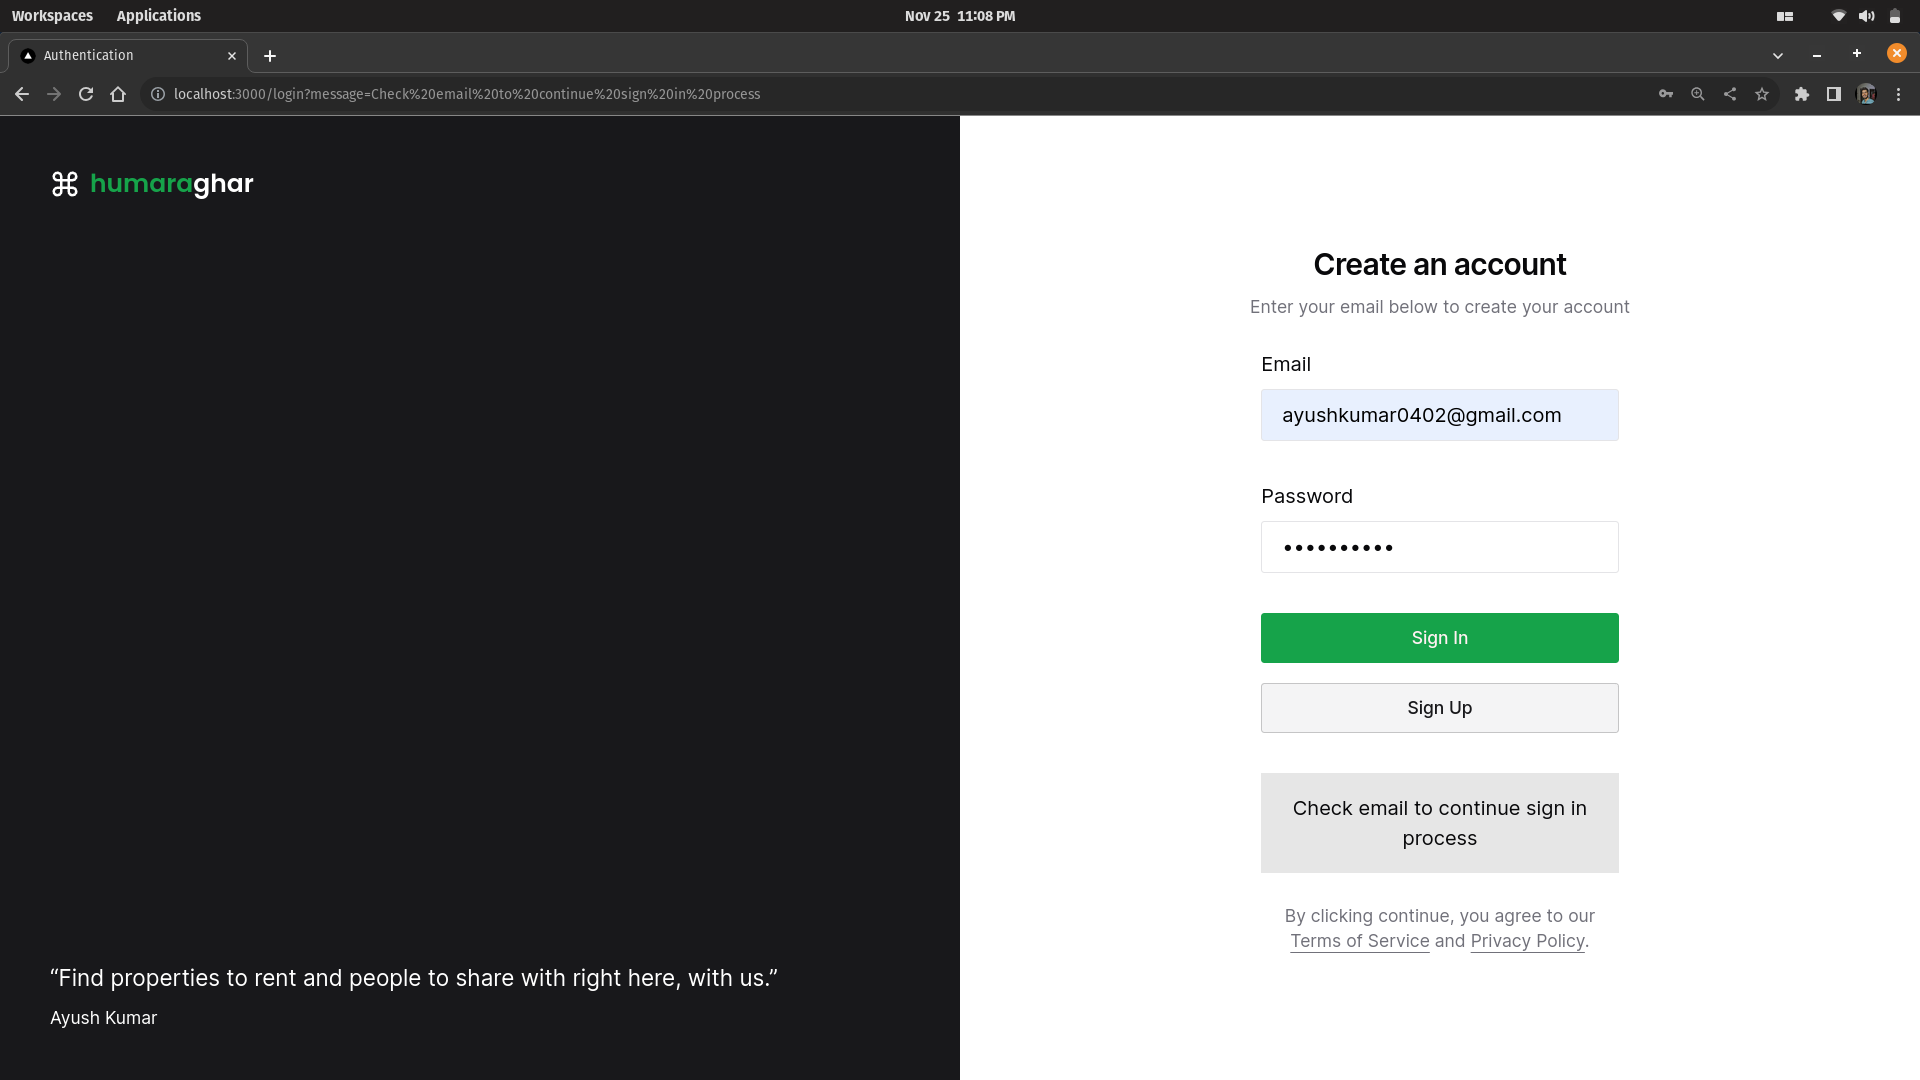
\includegraphics[width=0.9\textwidth]{Images/screenshots/signup.png}
    \caption{Login Page}
\end{figure}

On entering the correct details, a verification mail will be sent to the user’s email address. The user will have to
verify his/her email address to be able to login. The verification mail is shown in \par
\begin{figure}[h]
    \centering
    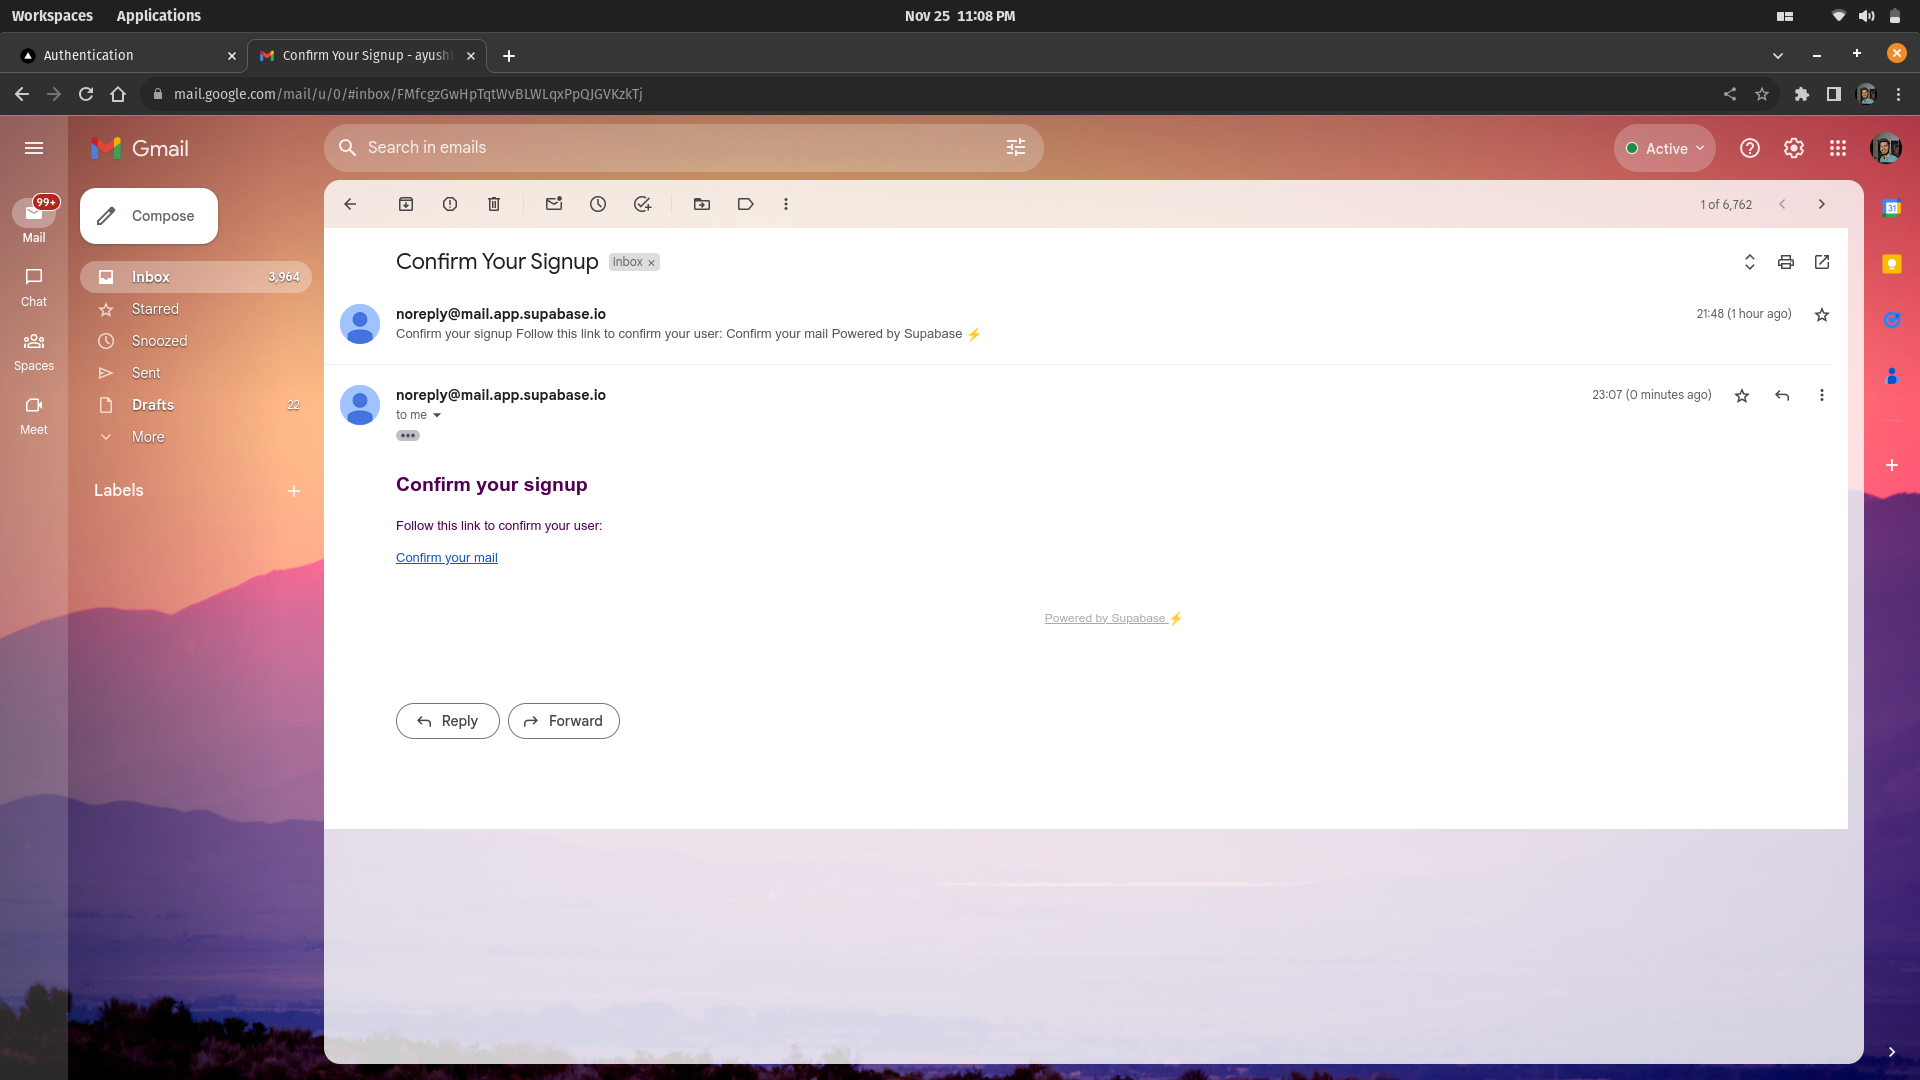
\includegraphics[width=0.8\textwidth]{Images/screenshots/mail.png}
    \caption{Verification Mail}
\end{figure}
\clearpage

\section{Onboarding Flow}
The onboarding flow contains forms containing user's data. The user will have to fill the forms to be able to use the
app. The first section of onboarding process aims to collect basic information about the user:

\begin{figure}[h]
    \centering
    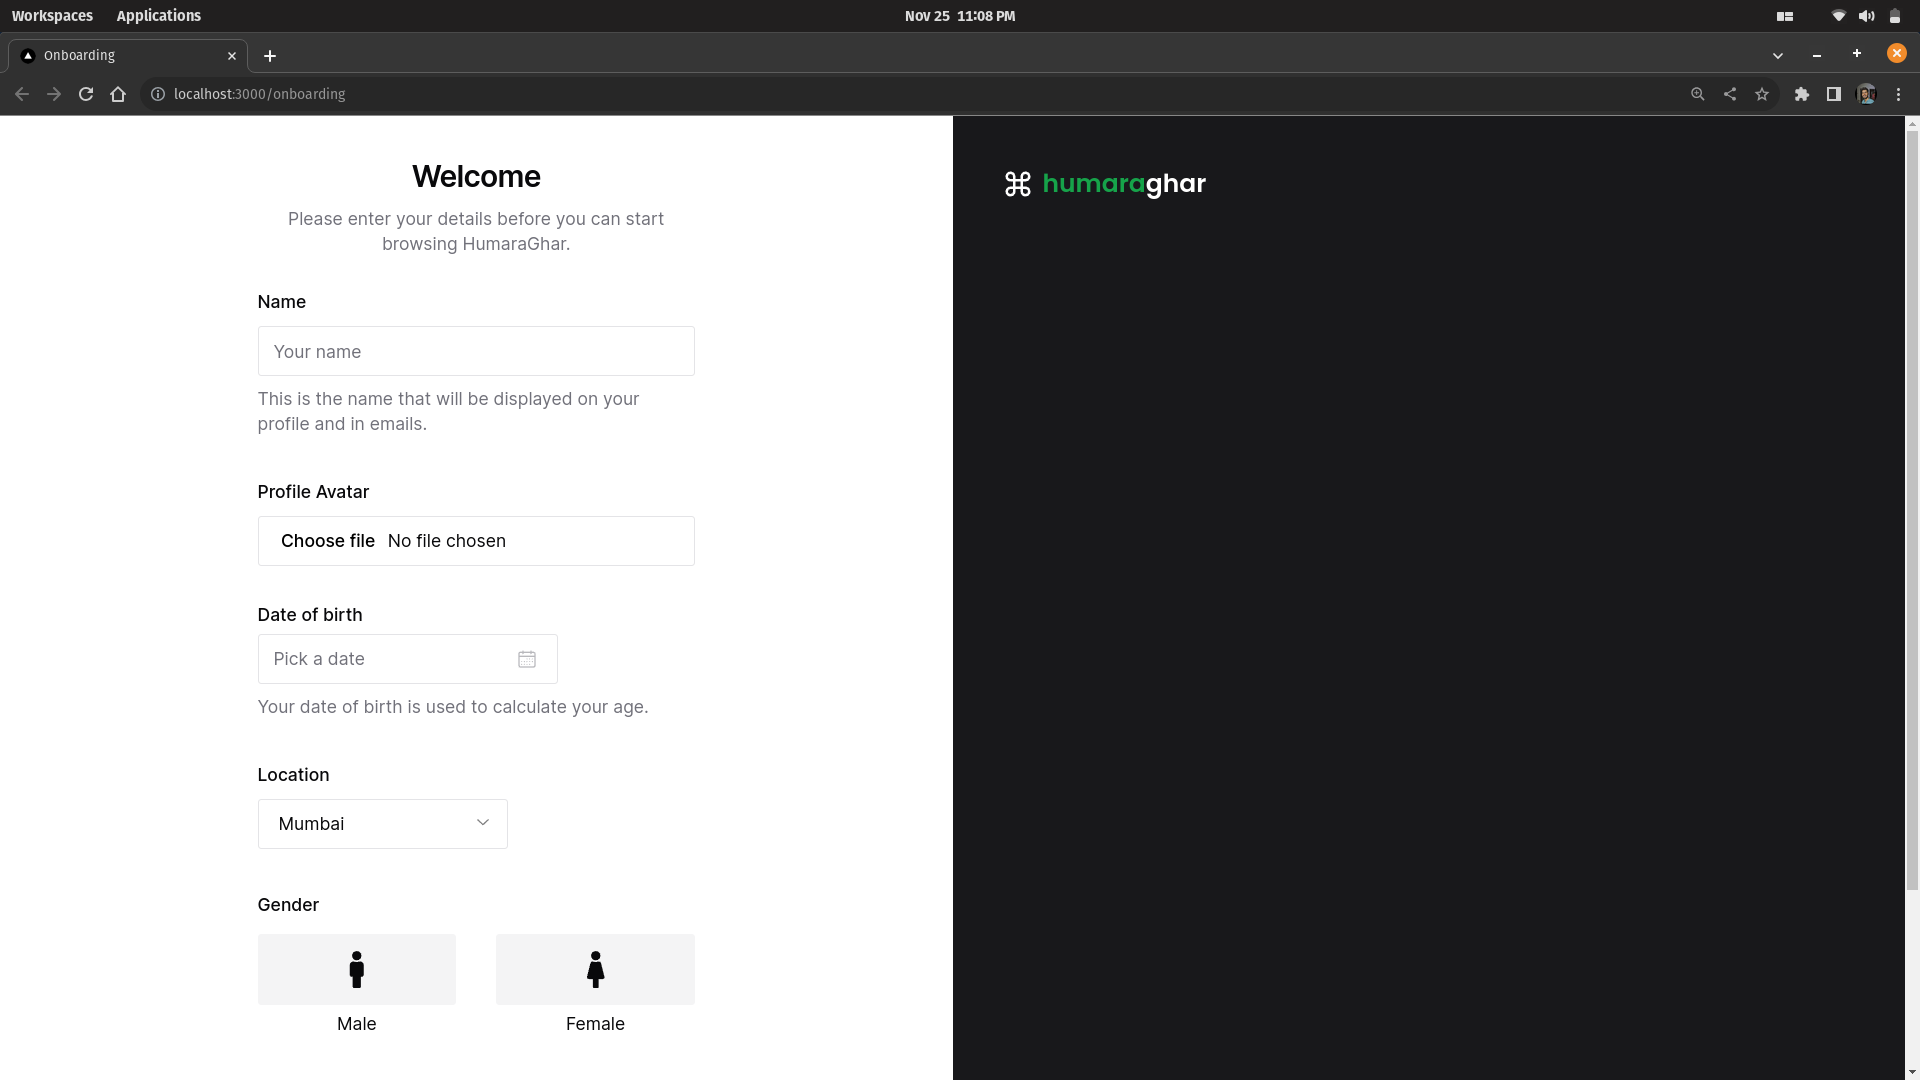
\includegraphics[width=0.8\textwidth]{Images/screenshots/onboarding.png}
    \caption{Onboarding Page 1}
\end{figure}

\par\noindent
The second section of onboarding process aims to collect information about the user's roommate preferences in case
he/she wants to share their room with someone else. The user can skip this section if he/she wants to live alone.
This data will be used to calculate match-score between users.\par
\begin{figure}[h]
    \centering
    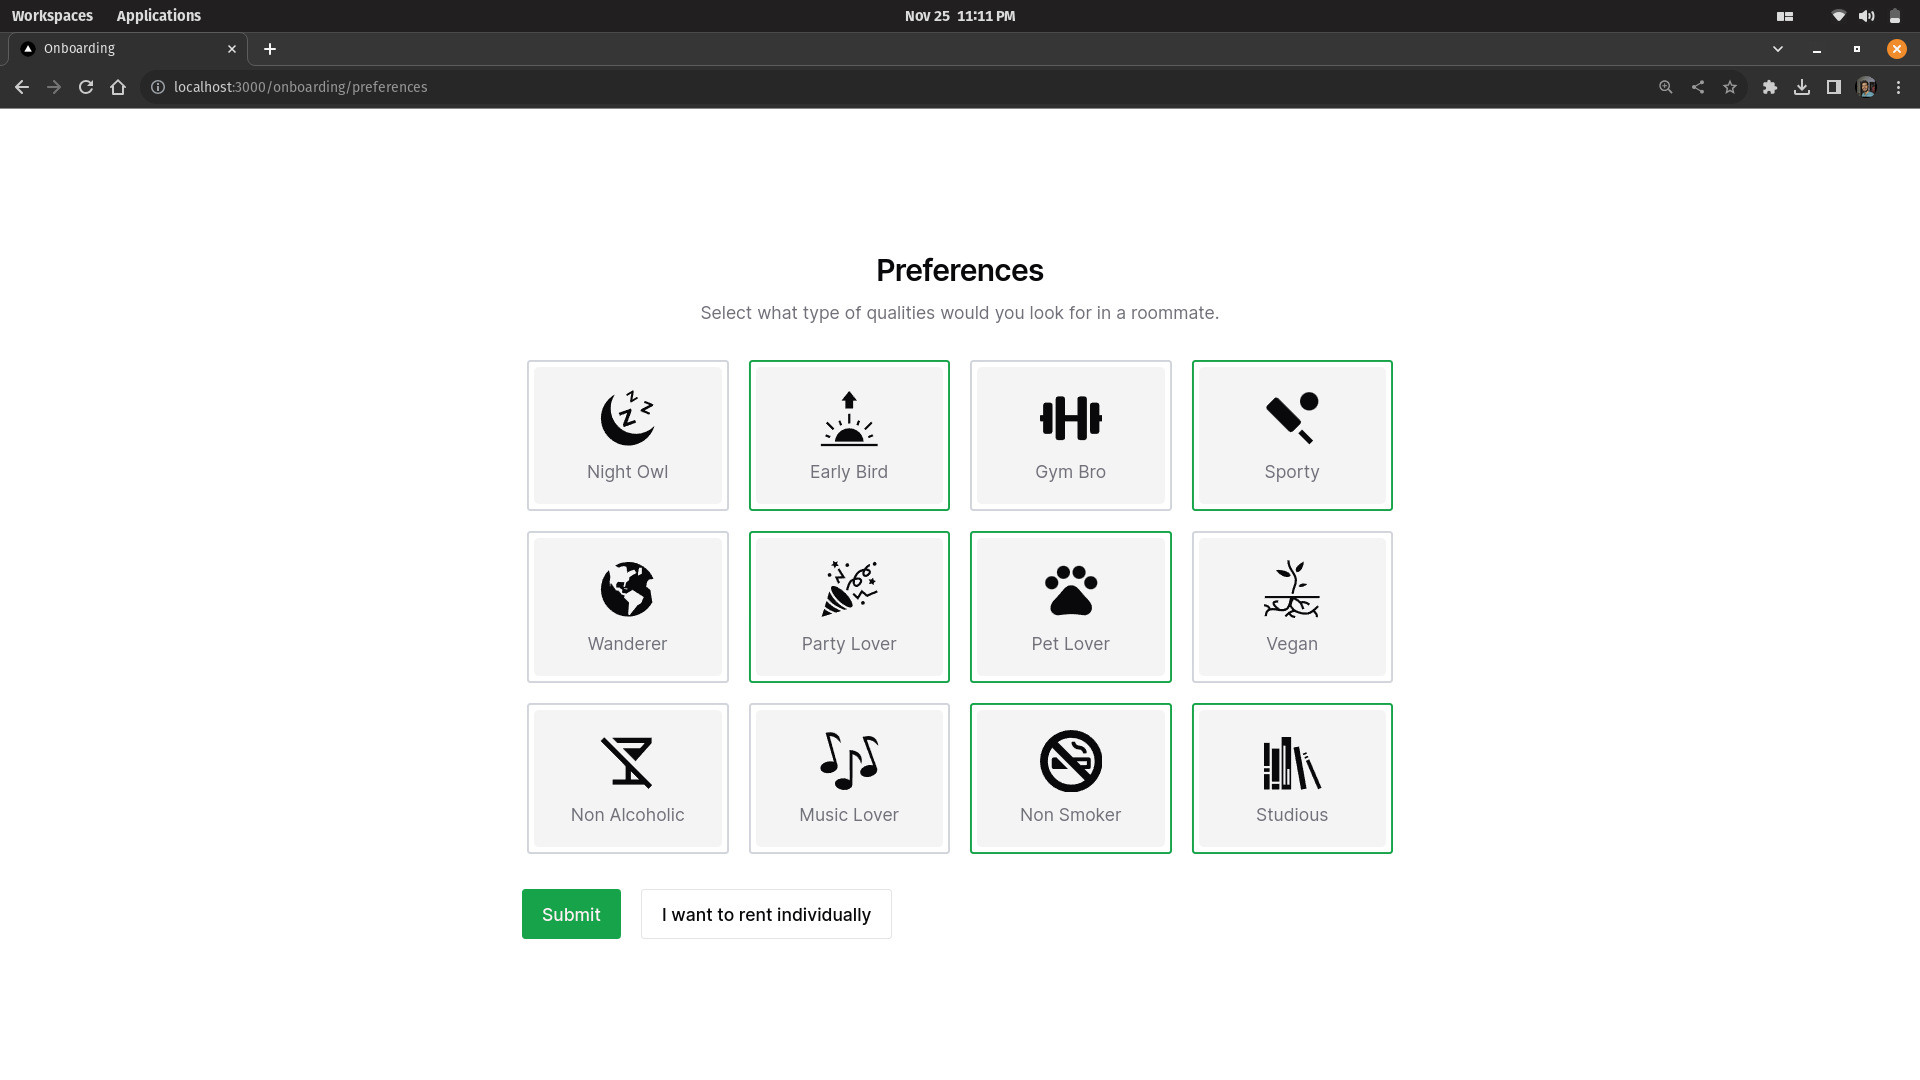
\includegraphics[width=0.8\textwidth]{Images/screenshots/preferences.png}
    \caption{Onboarding Page 2}
\end{figure}
\clearpage

\section{Dashboard}
The dashboard is the main page of the app. It contains various sections that will be discussed in detail in the
below.
\begin{figure}[h]
    \centering
    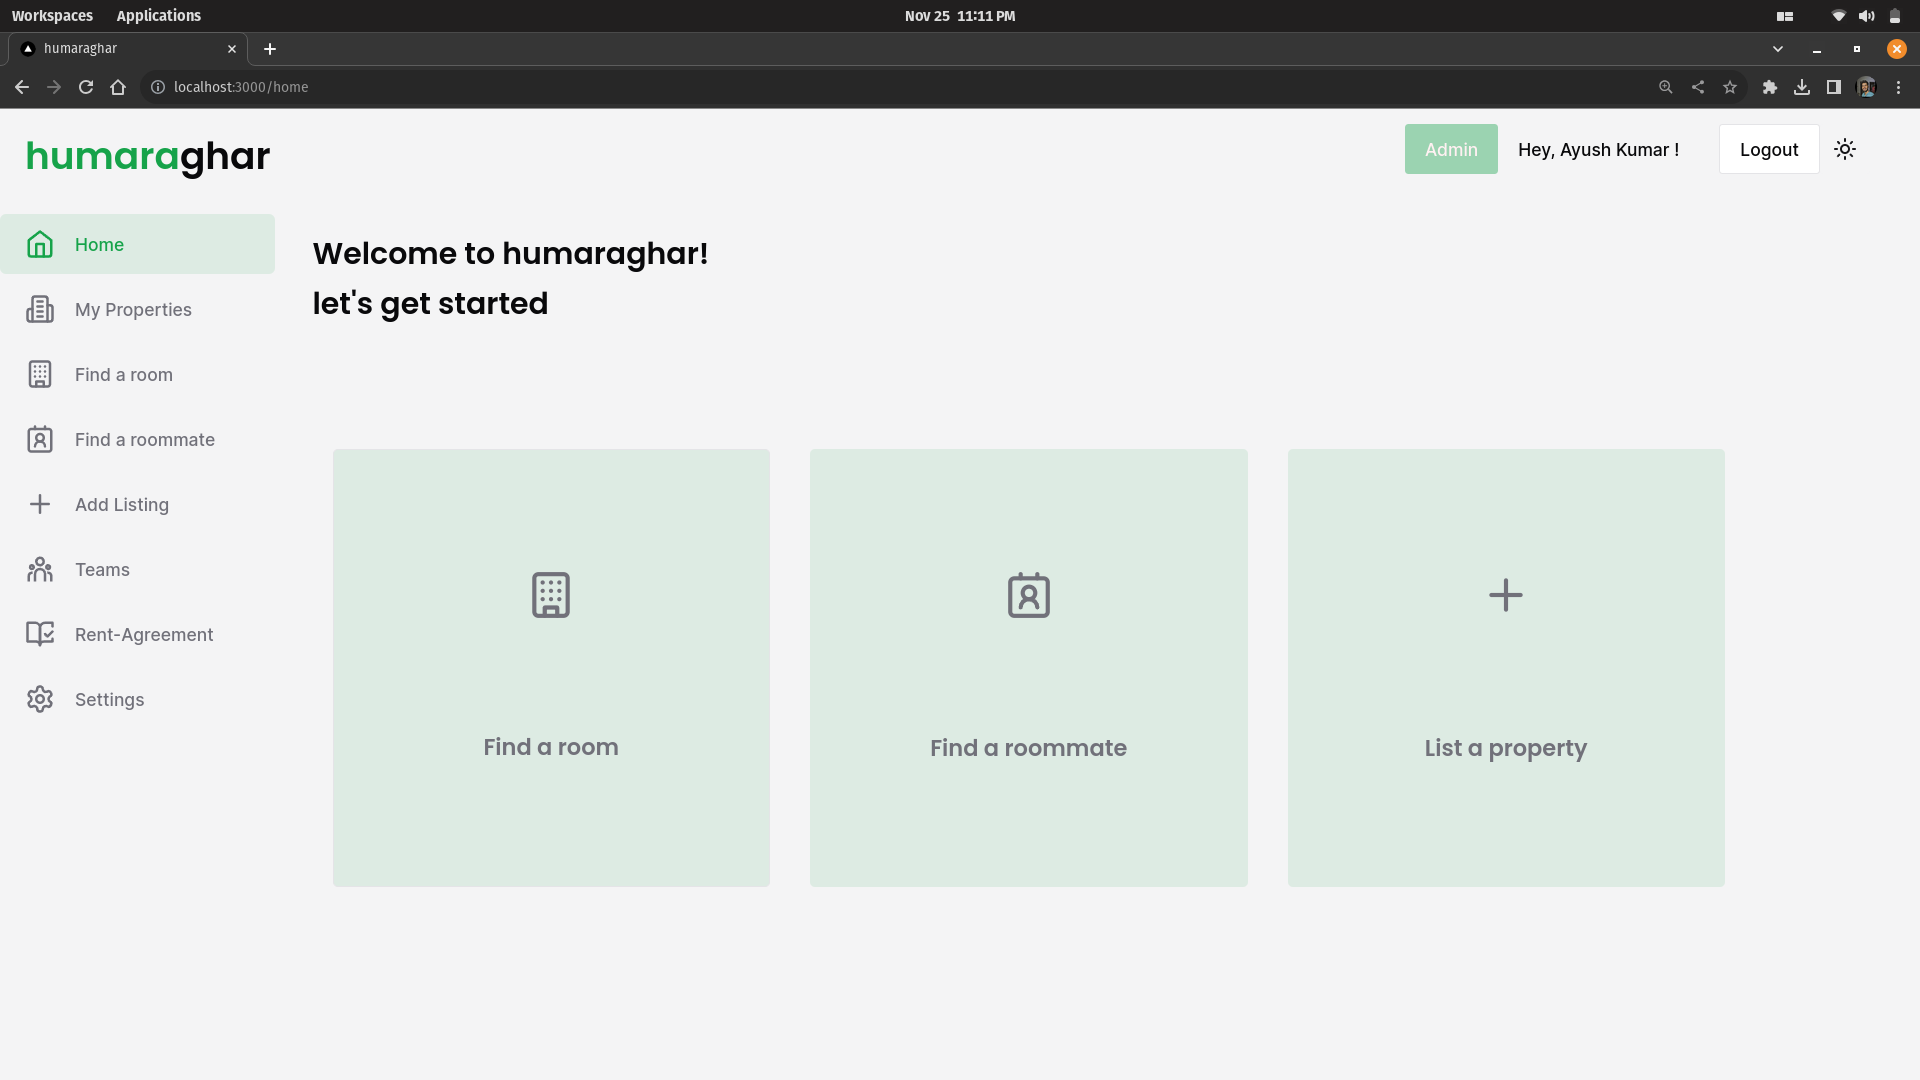
\includegraphics[width=0.8\textwidth]{Images/screenshots/home.png}
    \caption{Dashboard}
\end{figure}

The home page has links to redirect user to main parts of the dashboard catered towards finding a roommate and finding
a room. The user can also view his/her profile by clicking on the profile icon on the top right corner of the page.

\subsection{Find Roommate}
The find roommate page contains a list of all the users that have listing themselves as looking for a shared room, so anymore already having a place to live but looking for a roommate to split
the expenses can find them. Alternatively, you can also team-up among people looking for a room and search for an empty flat together. The user can filter the list based on
location and preferences.


\subsection{Find Room}
The find room page contains a list of all the users that have listing themselves as looking for a roommate, (already having a place to live). The user can filter the list based on
location and preferences again. The rooms which are not shared are also listed here. The user can also view them.

\begin{figure}[h]
    \centering
    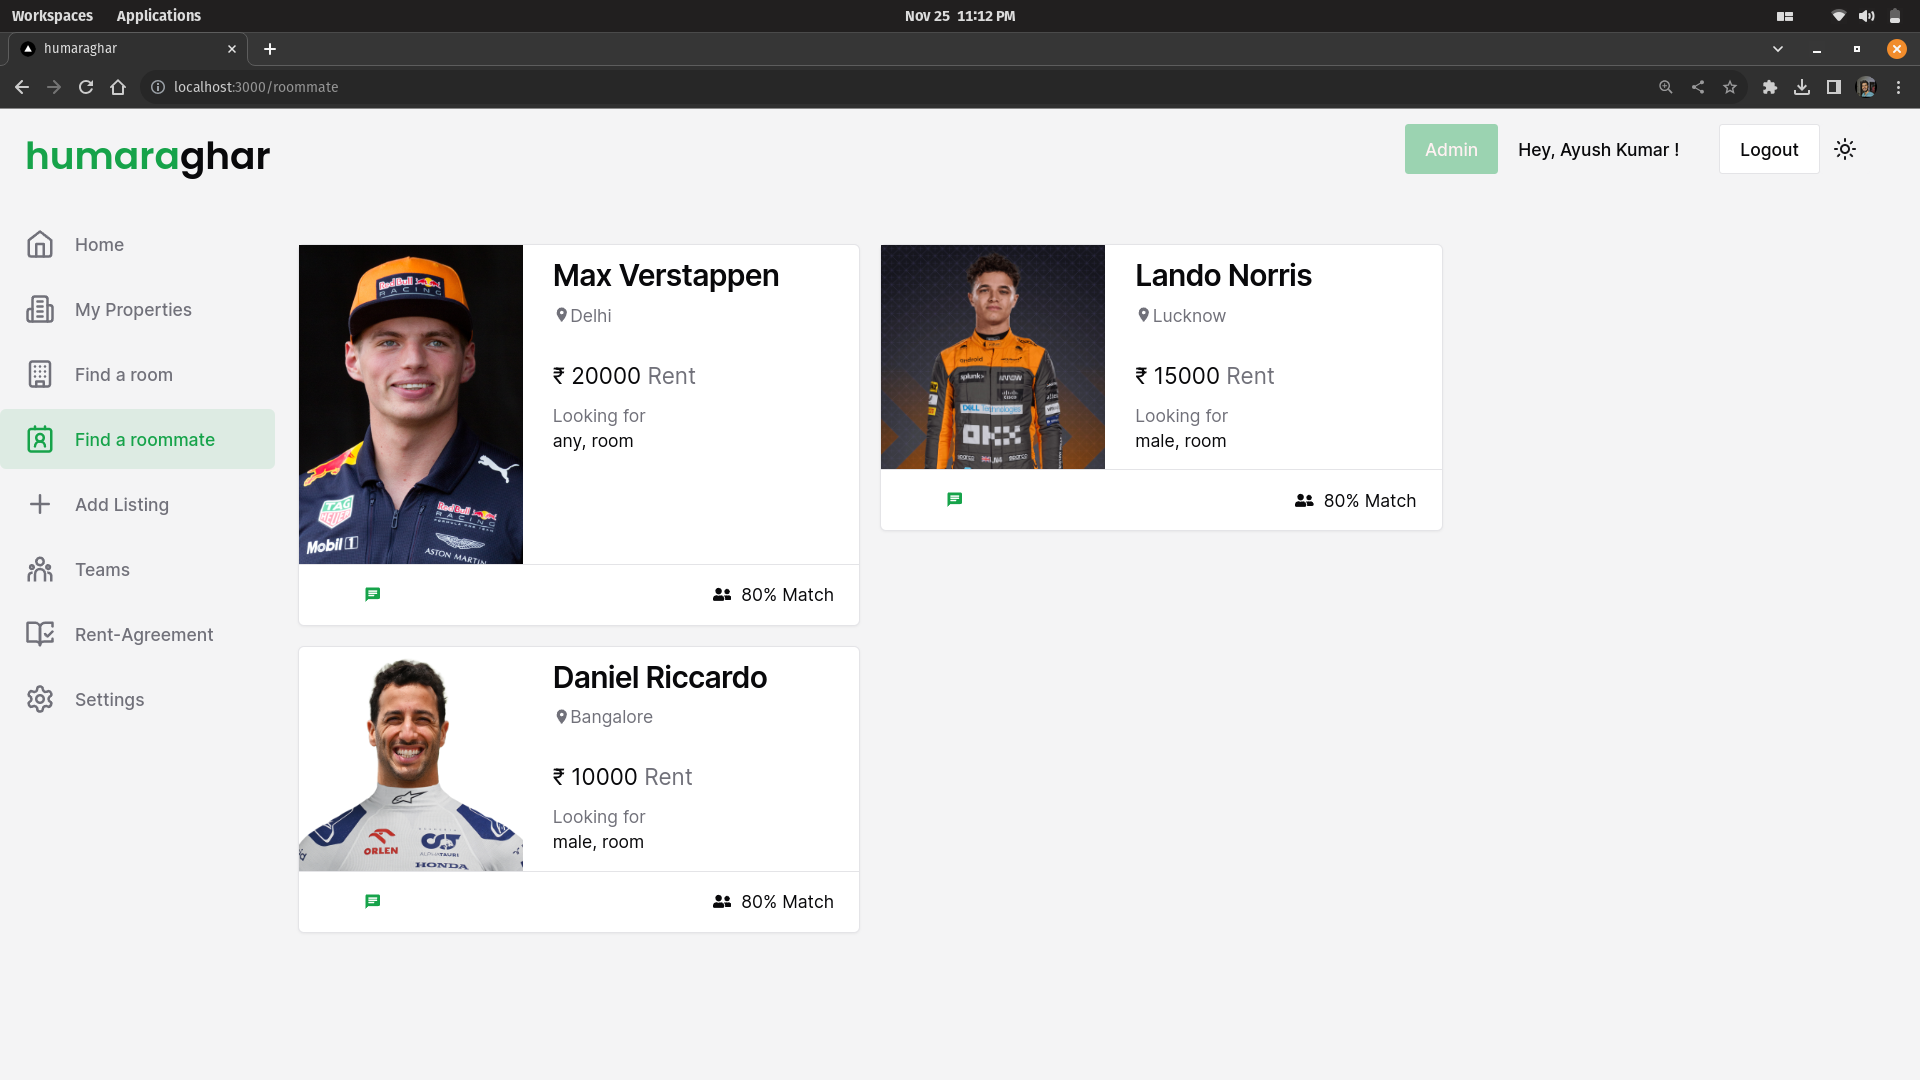
\includegraphics[width=1\textwidth]{Images/screenshots/roommates.png}
    \caption{Find Roommate}
\end{figure}

\begin{figure}[h]
    \centering
    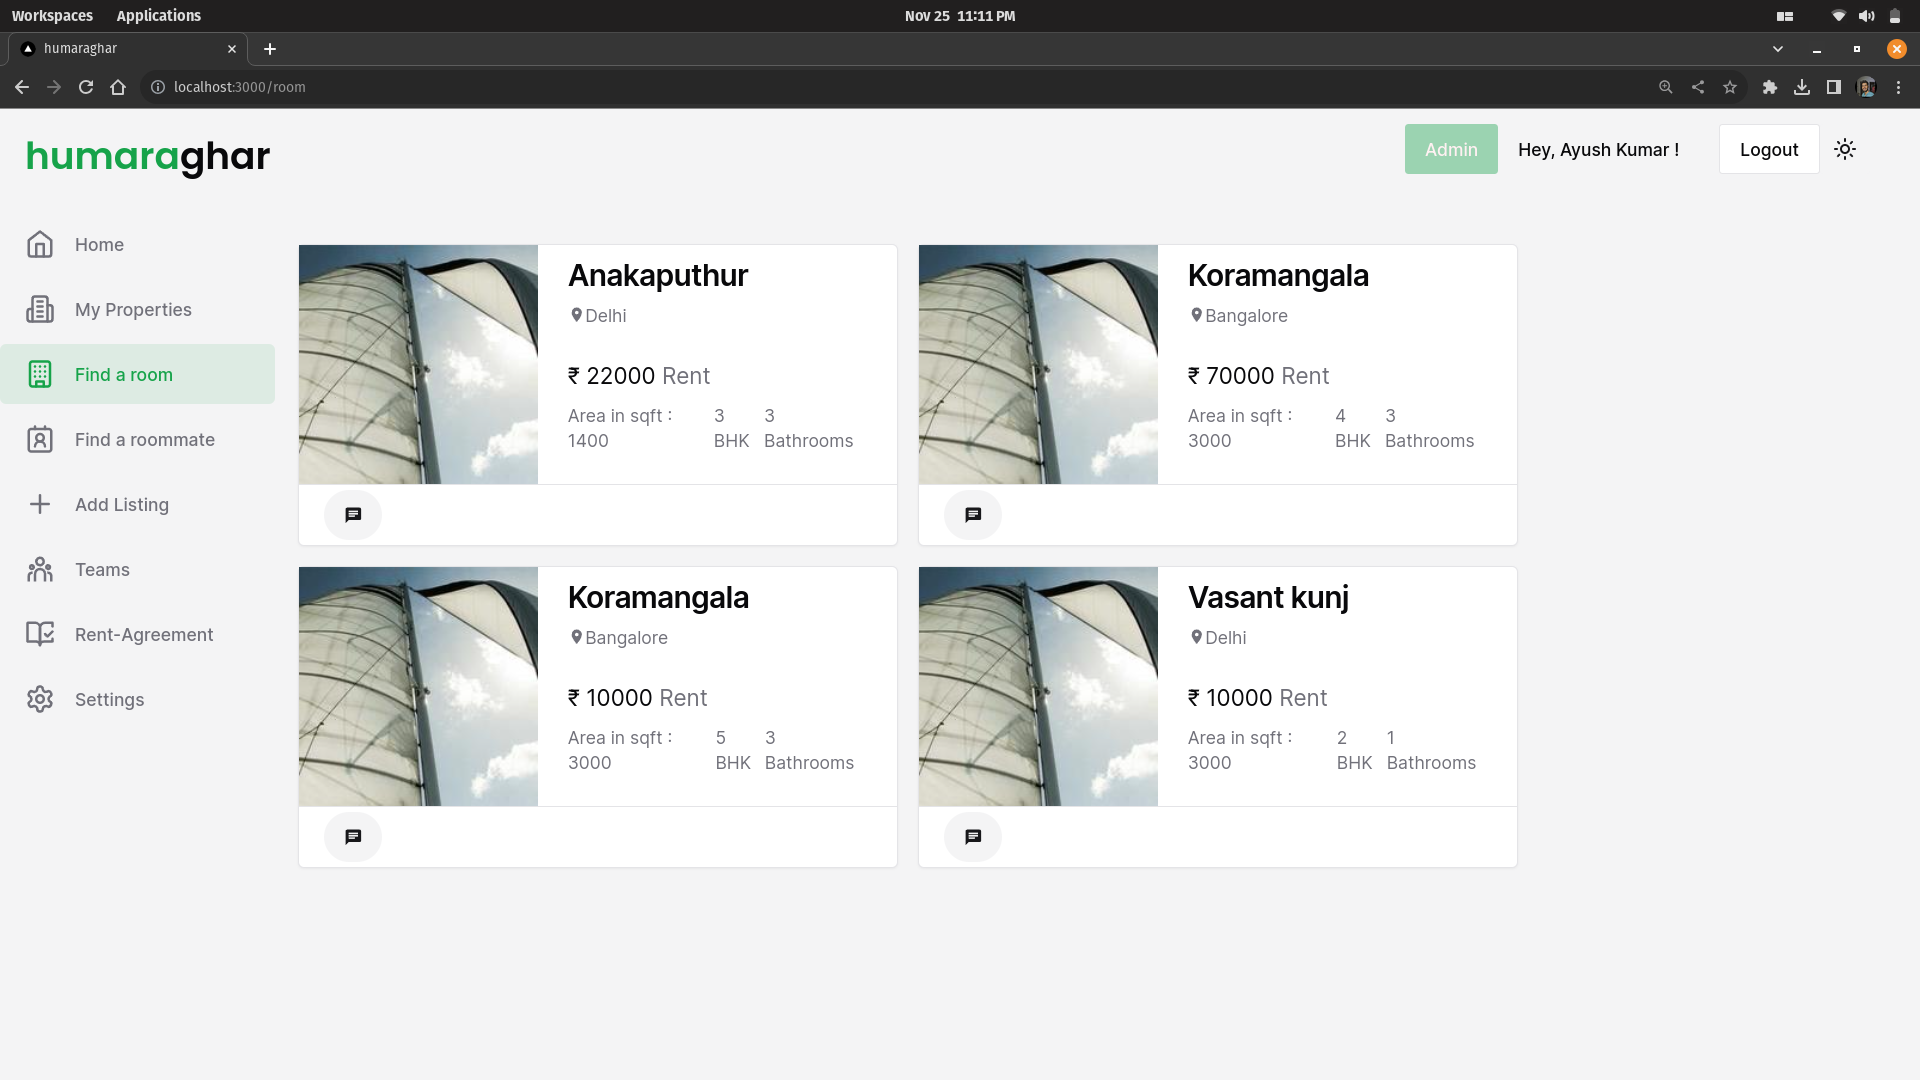
\includegraphics[width=1\textwidth]{Images/screenshots/rooms.png}
    \caption{Find Room}
\end{figure}

\clearpage

The user can either view the detailed description of the room or the roommate by clicking the card. Or he/she can
directly mark themselves interested in the property by clicking the interested button. It will prompt the user to select
if they are interested as a team (if part of any) or individually.

\begin{figure}[h]
    \centering
    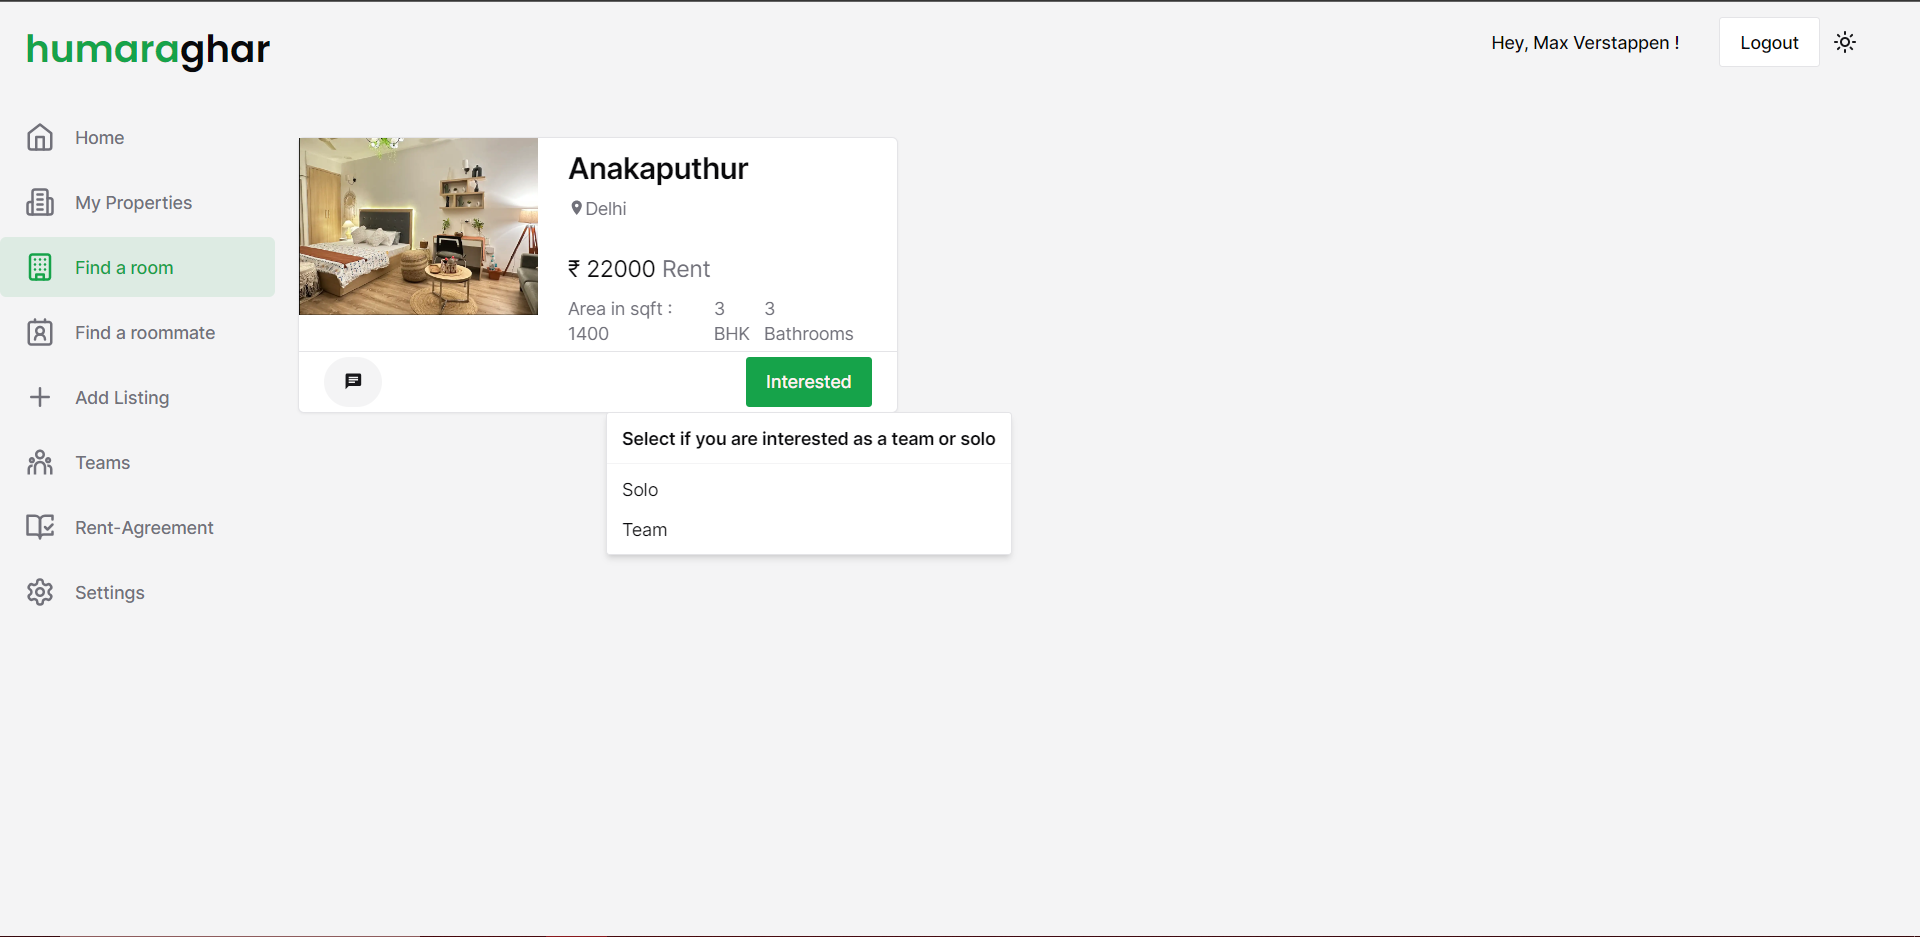
\includegraphics[width=0.8\textwidth]{Images/screenshots/interestedas.PNG}
    \caption{Interested As}
\end{figure}

Clicking as interested would notify the poster and then they can initiate a chat if they are willing to proceed further.
\begin{figure}[h]
    \centering
    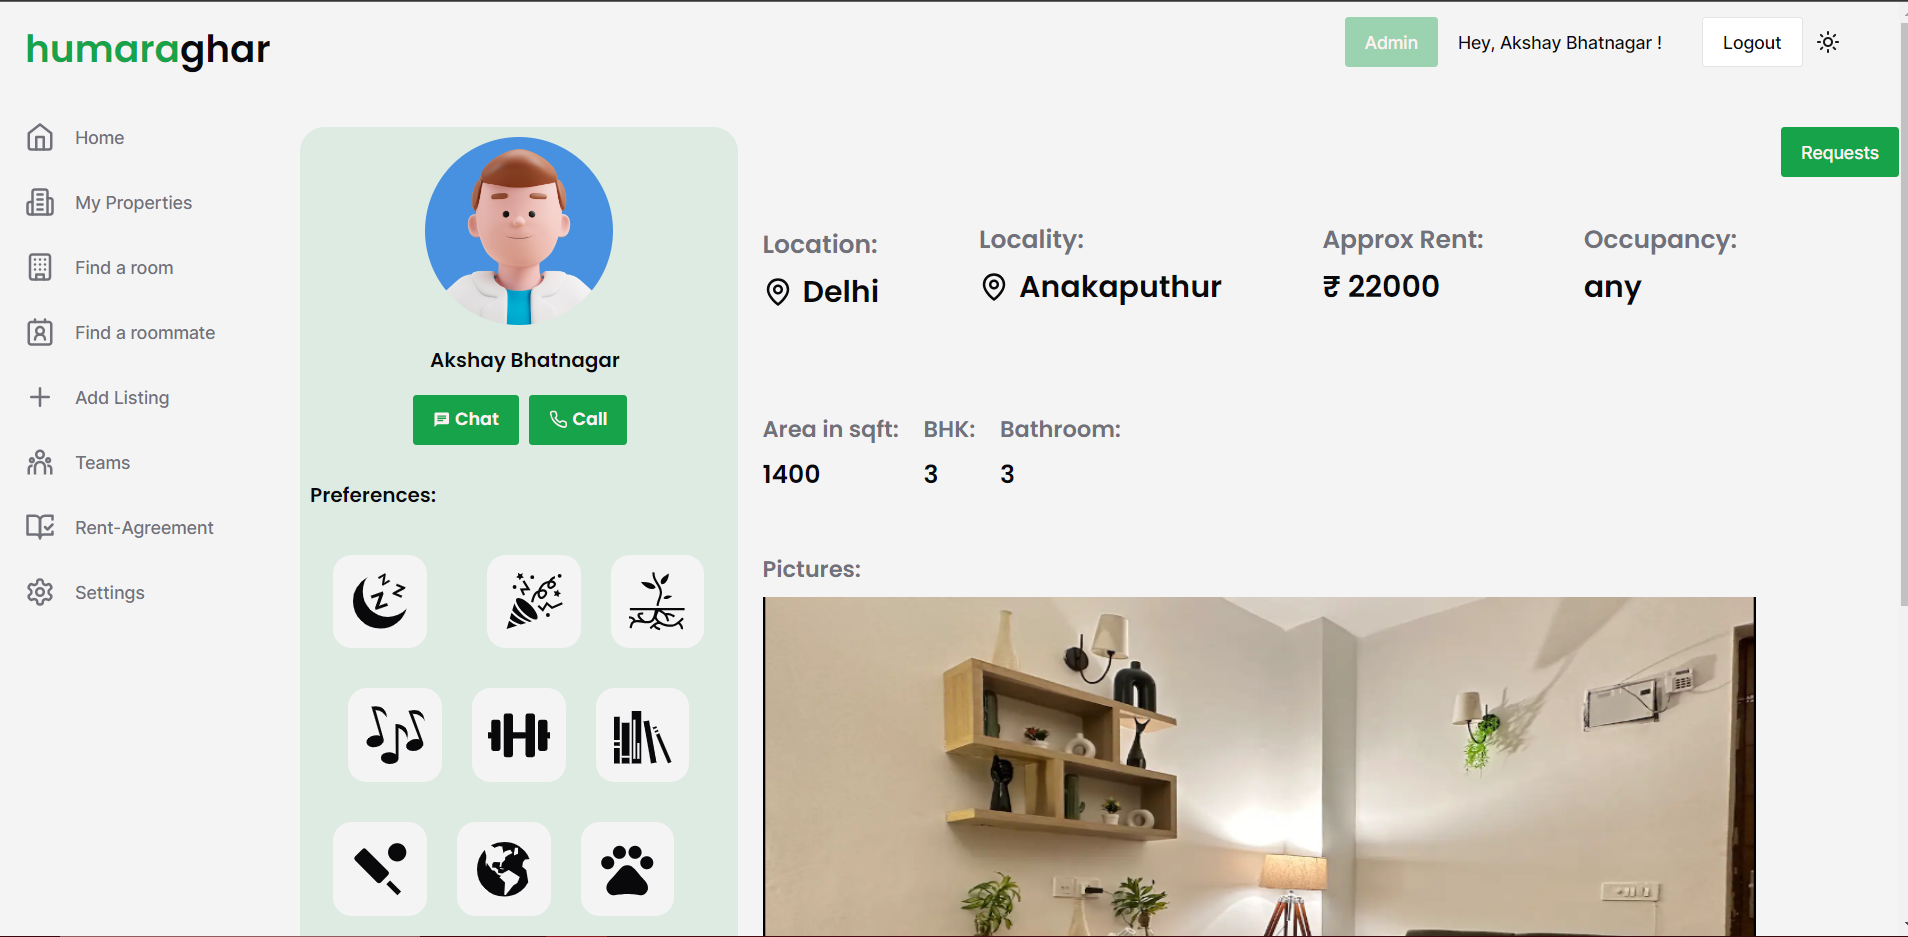
\includegraphics[width=0.8\textwidth]{Images/screenshots/userpage.PNG}
    \caption{Details Page}
\end{figure}
\clearpage

\subsection{Add Listing}
The add listing page is used to add a new listing to the database. The user can add a listing for wanting to share their room, find a new room or rent their property.
\begin{figure}[h]
    \centering
    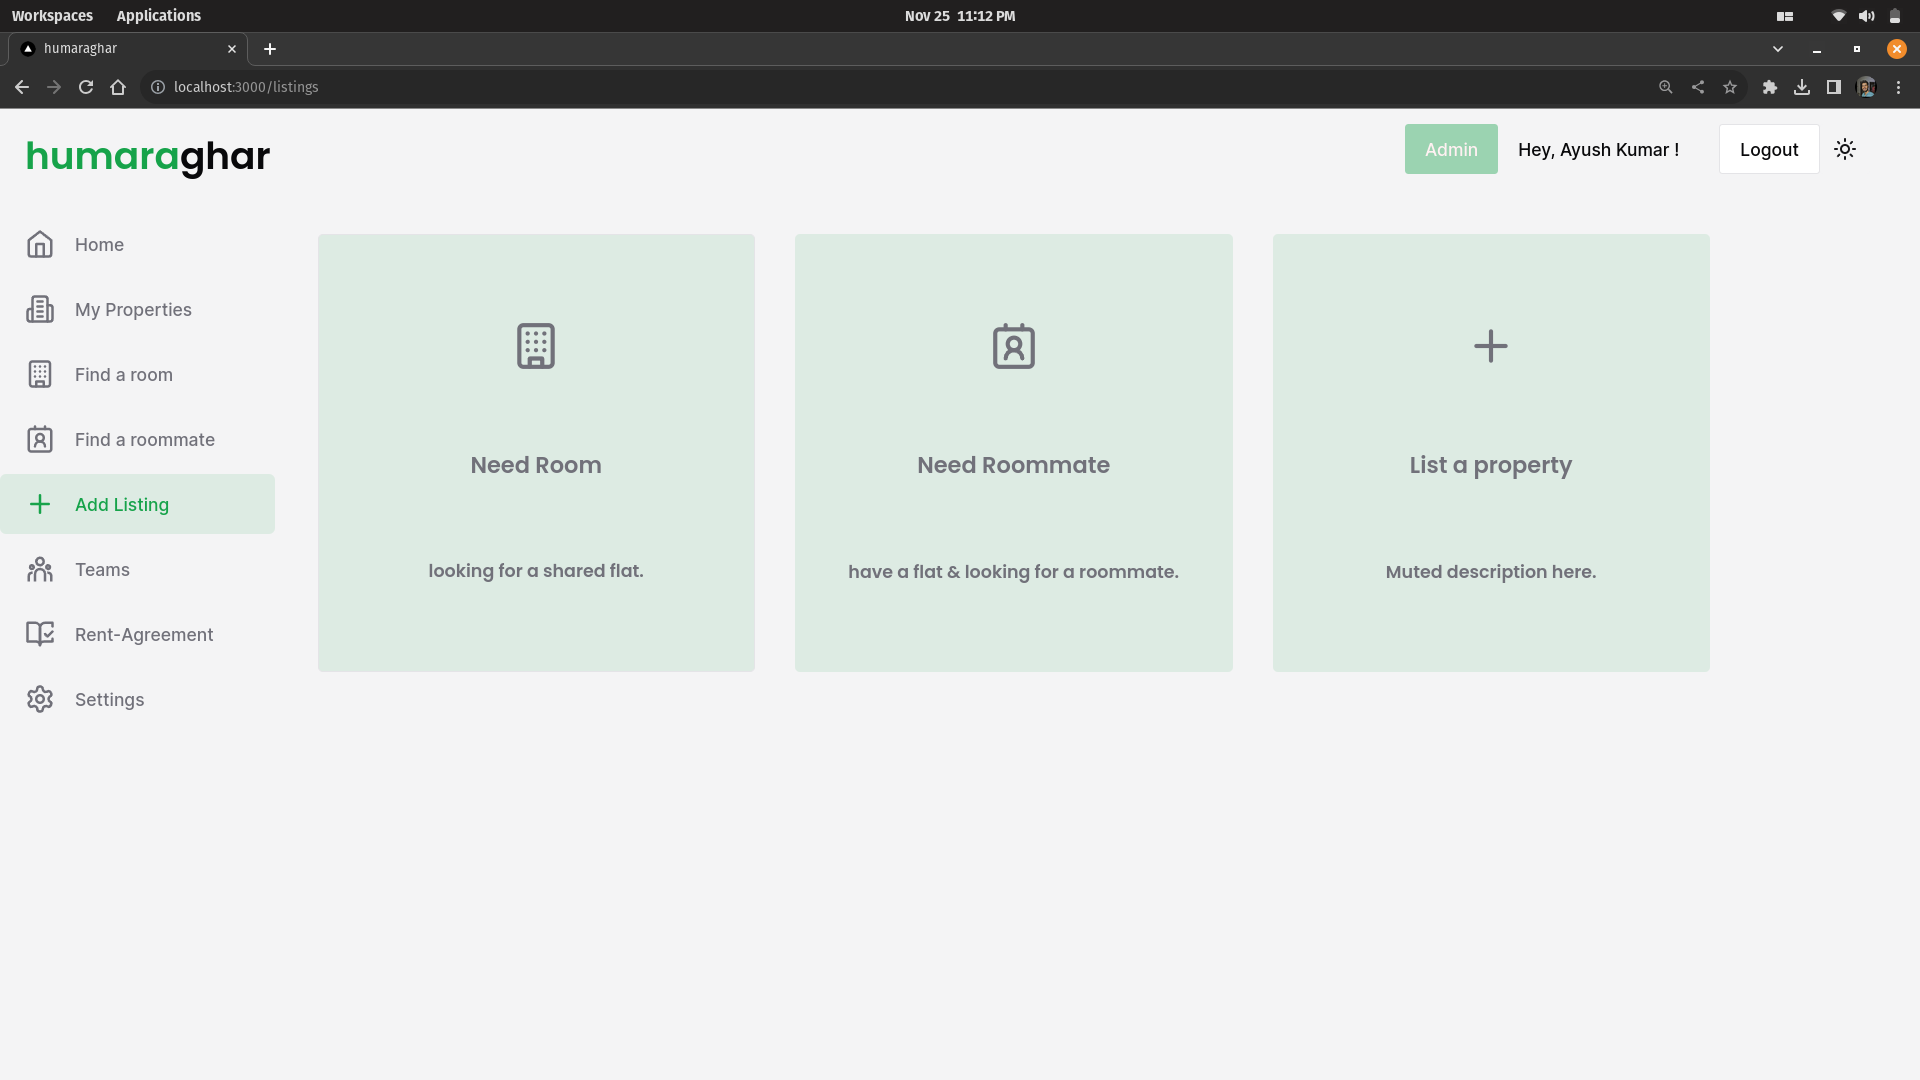
\includegraphics[width=0.8\textwidth]{Images/screenshots/addlisting.png}
    \caption{Add Listing}
\end{figure}

\noindent Choosing any option will take you to a form where you can fill in the details of the listing.
The form for adding a property listing is shown here \par
\begin{figure}[h]
    \centering
    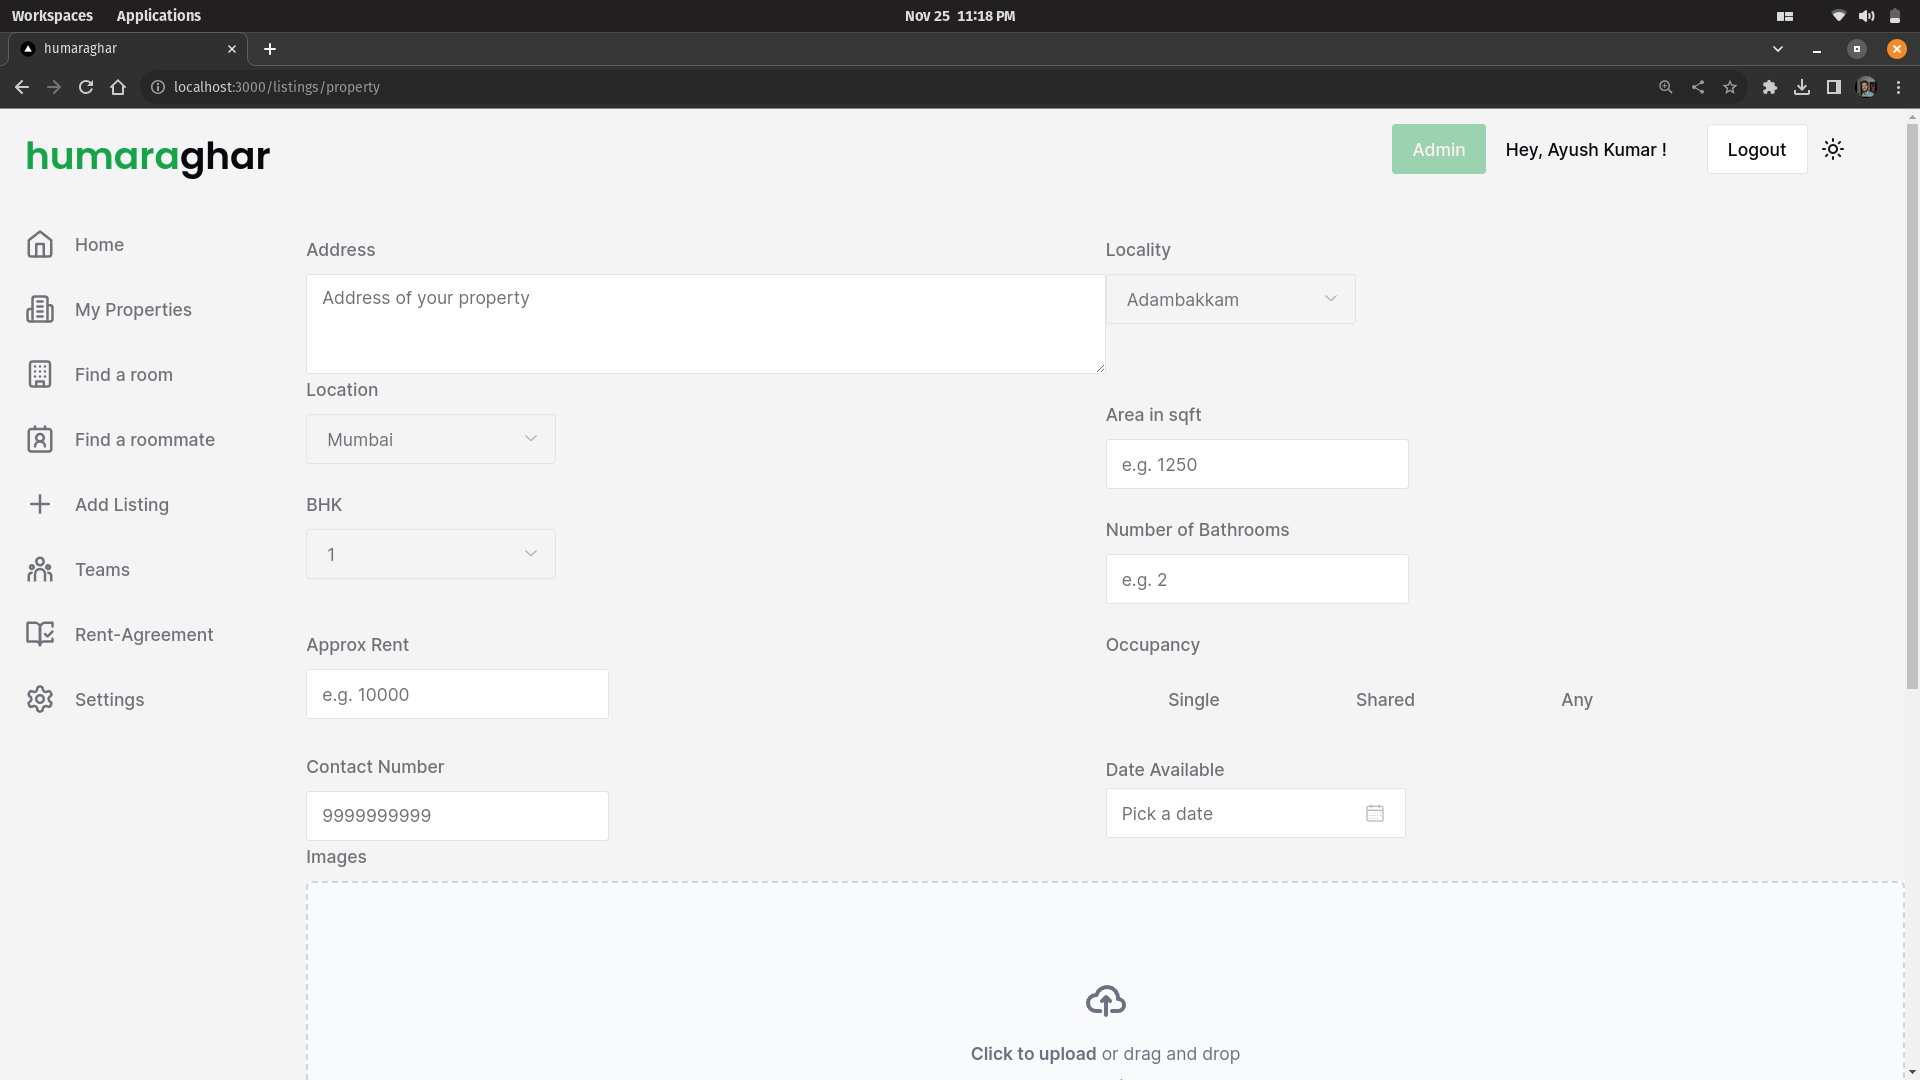
\includegraphics[width=0.8\textwidth]{Images/screenshots/proplisting.png}
    \caption{Add Room}
\end{figure}

\clearpage

\subsection{Team Management}
The team management page is used to manage the teams that the user is a part of. The user can view the team that he/she is a part of or create a new team. The user can also view their sent invites and received invites
with option to accept or decline them.
\begin{figure}[h]
    \centering
    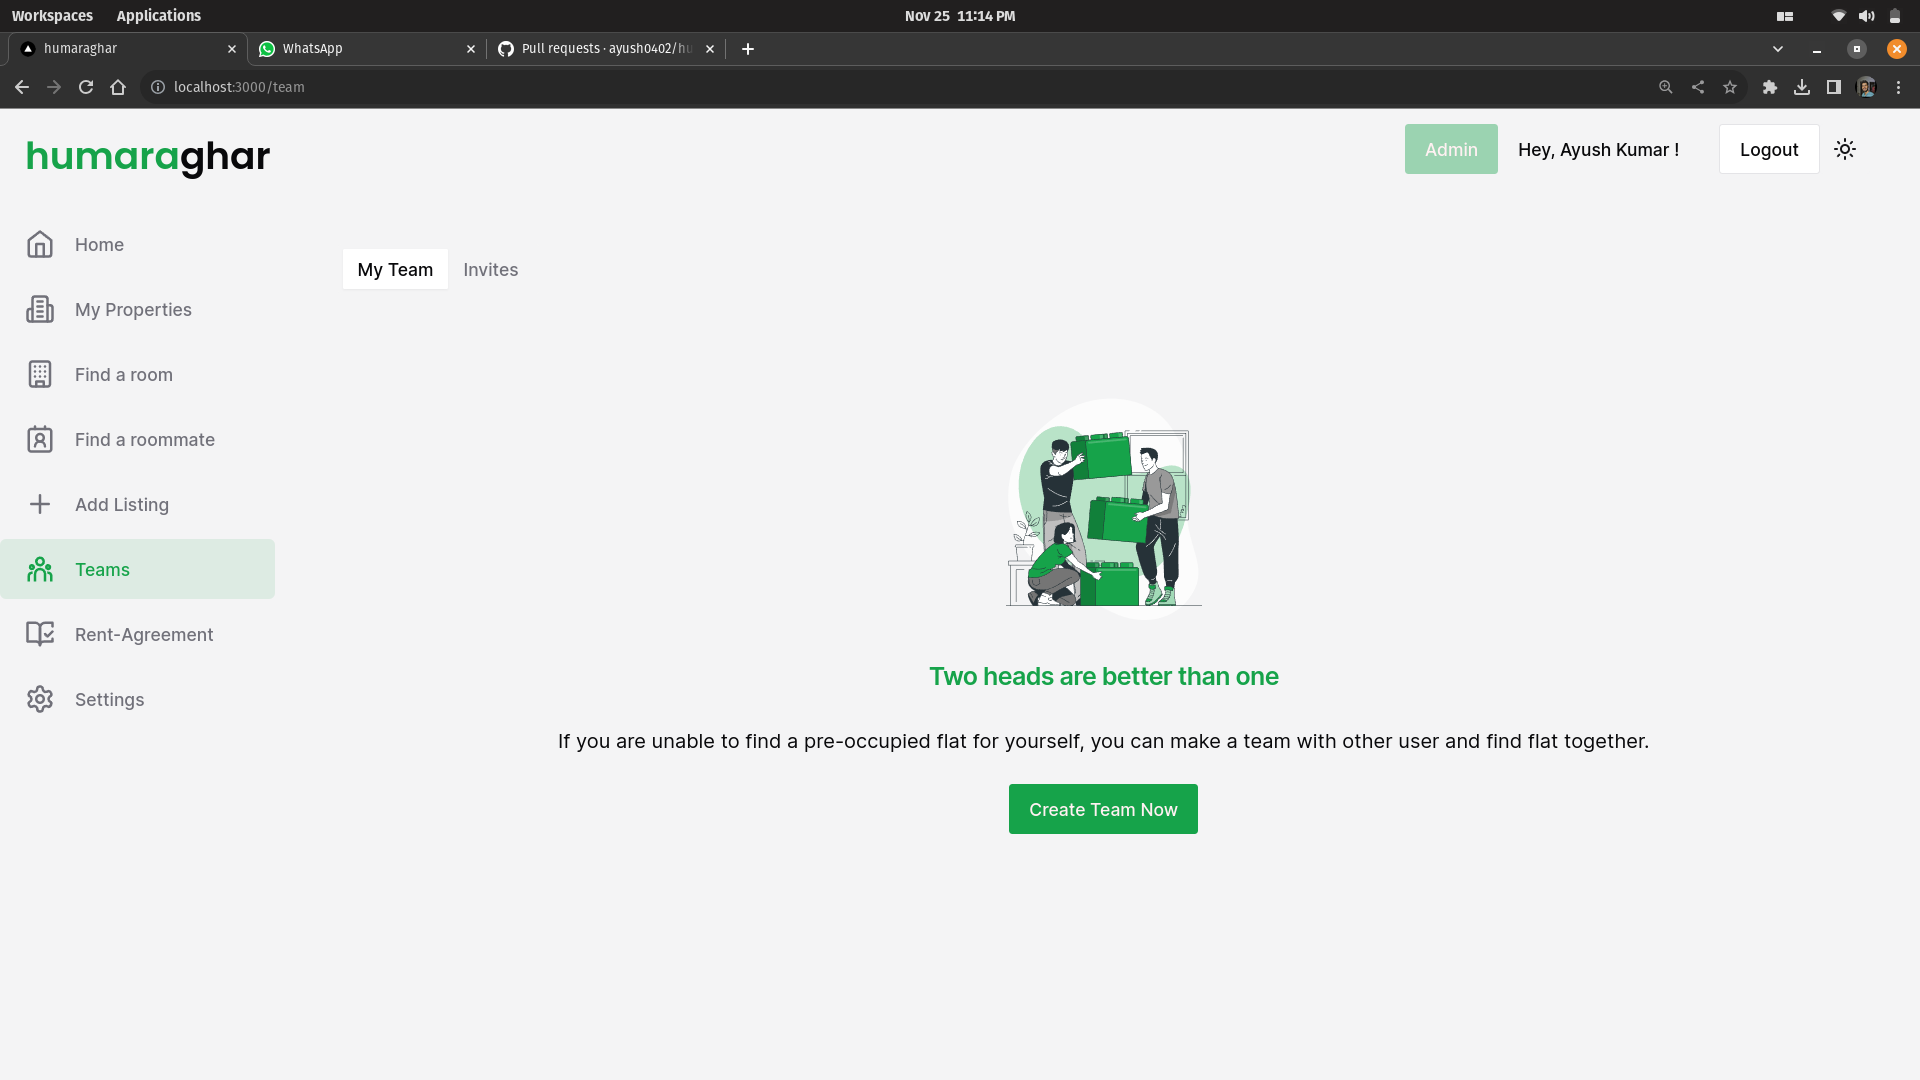
\includegraphics[width=0.8\textwidth]{Images/screenshots/createteam.png}
    \caption{Create Team}
\end{figure}

\begin{figure}[h]
    \centering
    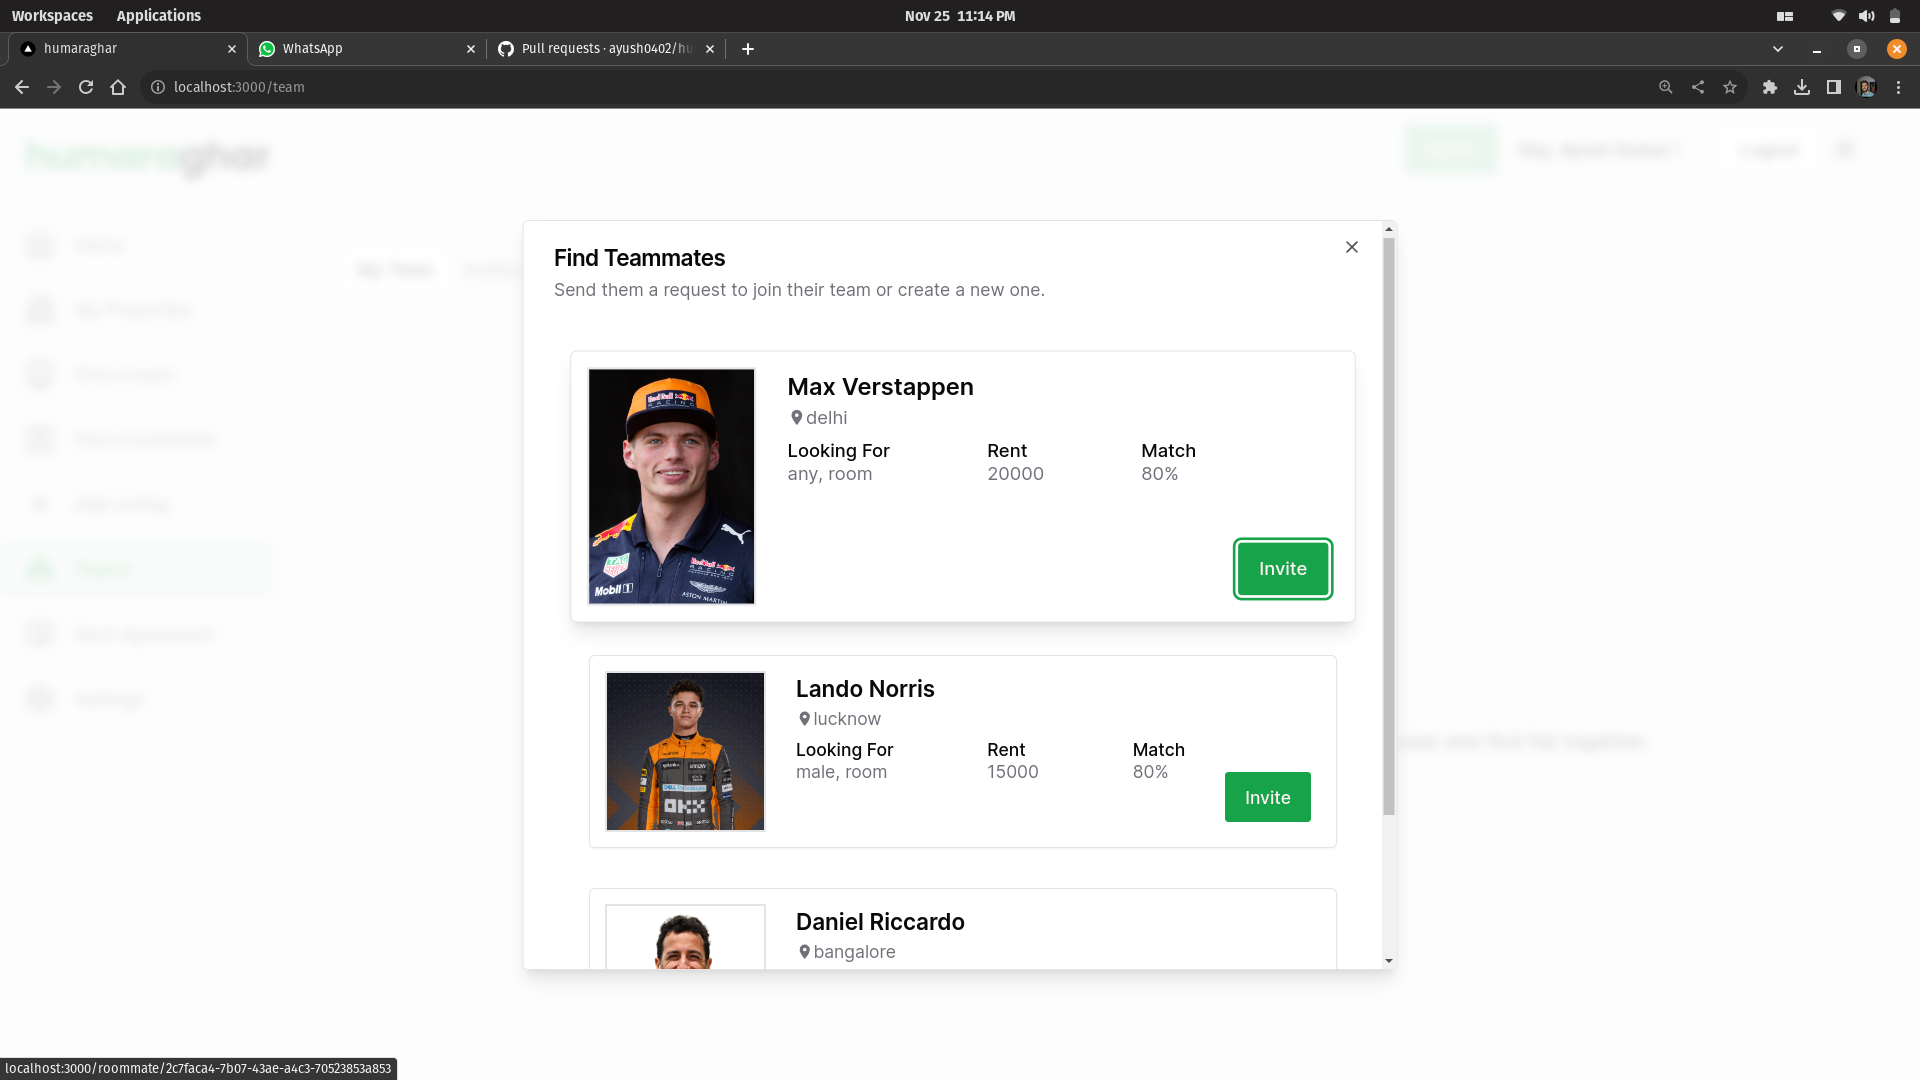
\includegraphics[width=0.8\textwidth]{Images/screenshots/teampopup.png}
    \caption{Team Invite Popup}
\end{figure}

\begin{figure}[h]
    \centering
    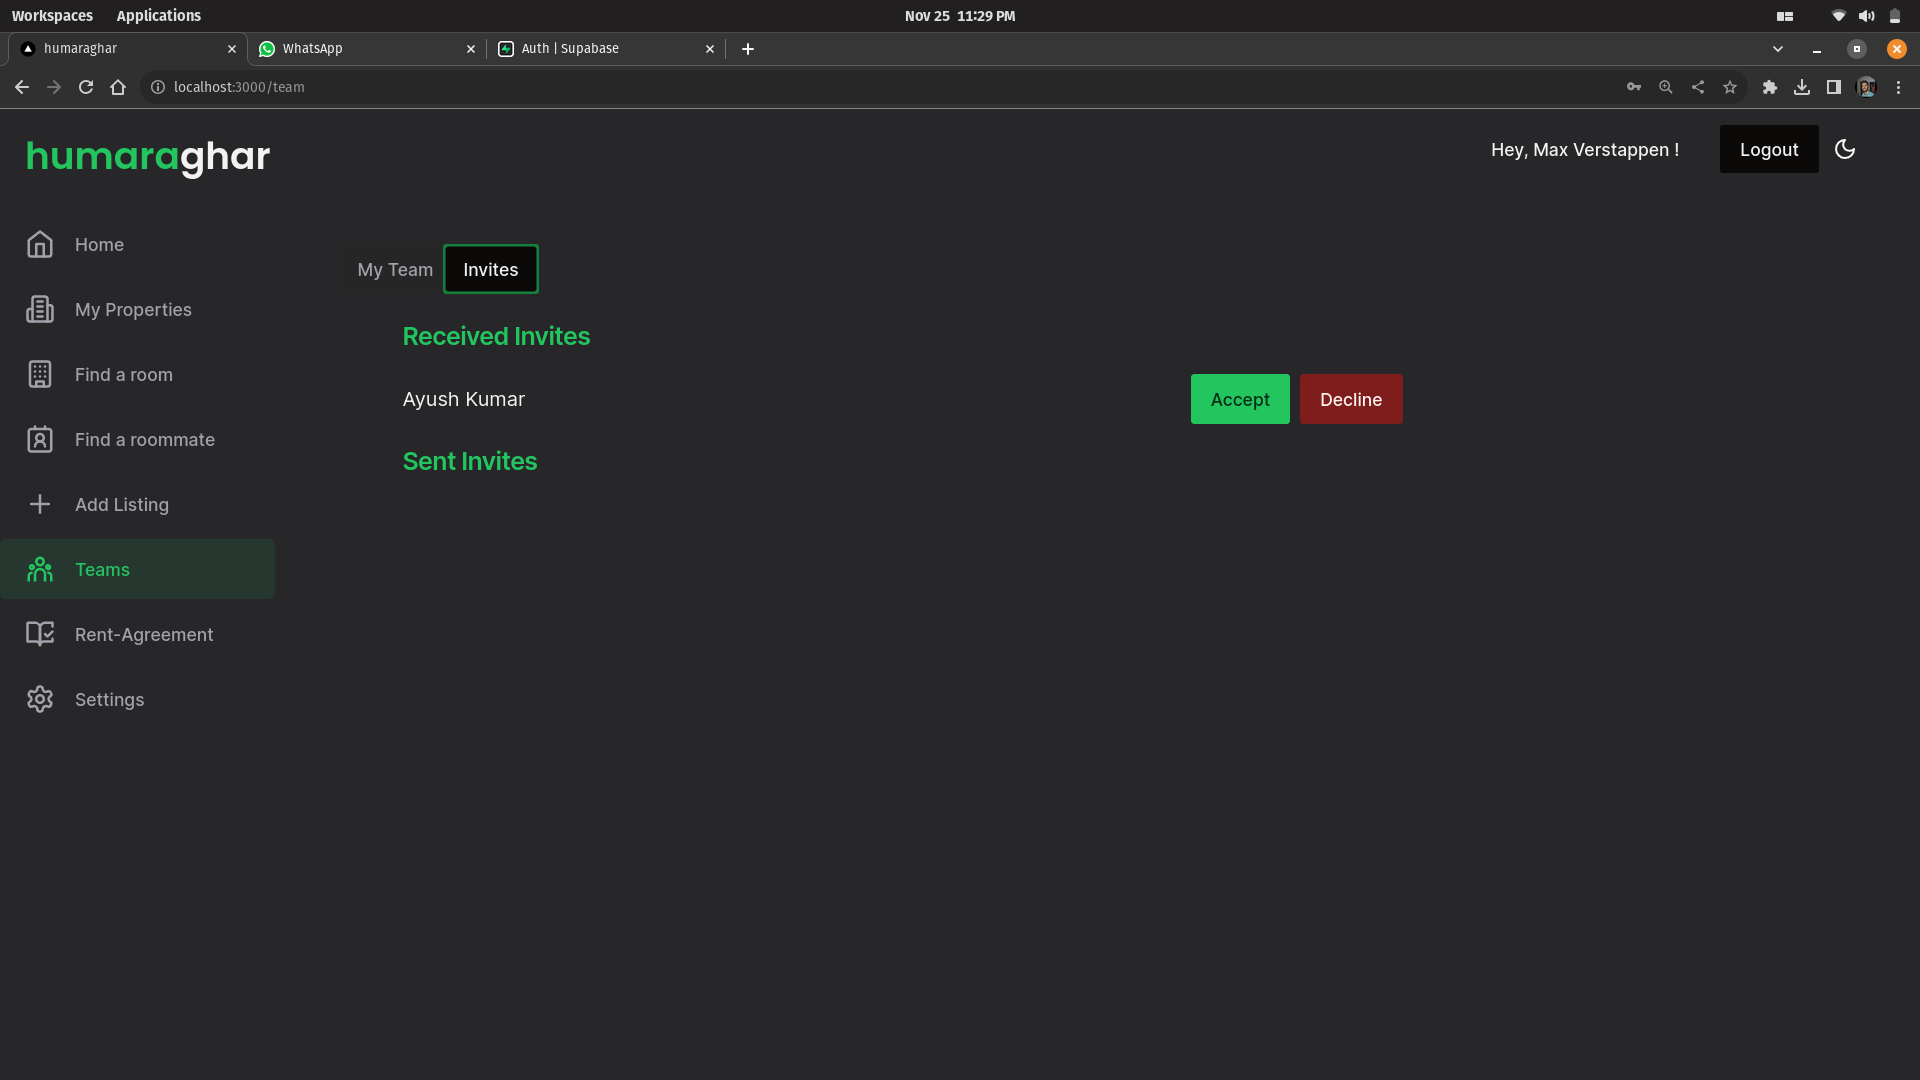
\includegraphics[width=0.8\textwidth]{Images/screenshots/invites.png}
    \caption{Pending Invites}
\end{figure}

\par\bigskip\bigskip
\subsection{Rent Agreement Generation}{
    The rent agreement generation page is used to generate a rent agreement for the user. The user can fill in the details of the agreement and generate a pdf of the agreement.
    \begin{figure}[h]
        \centering
        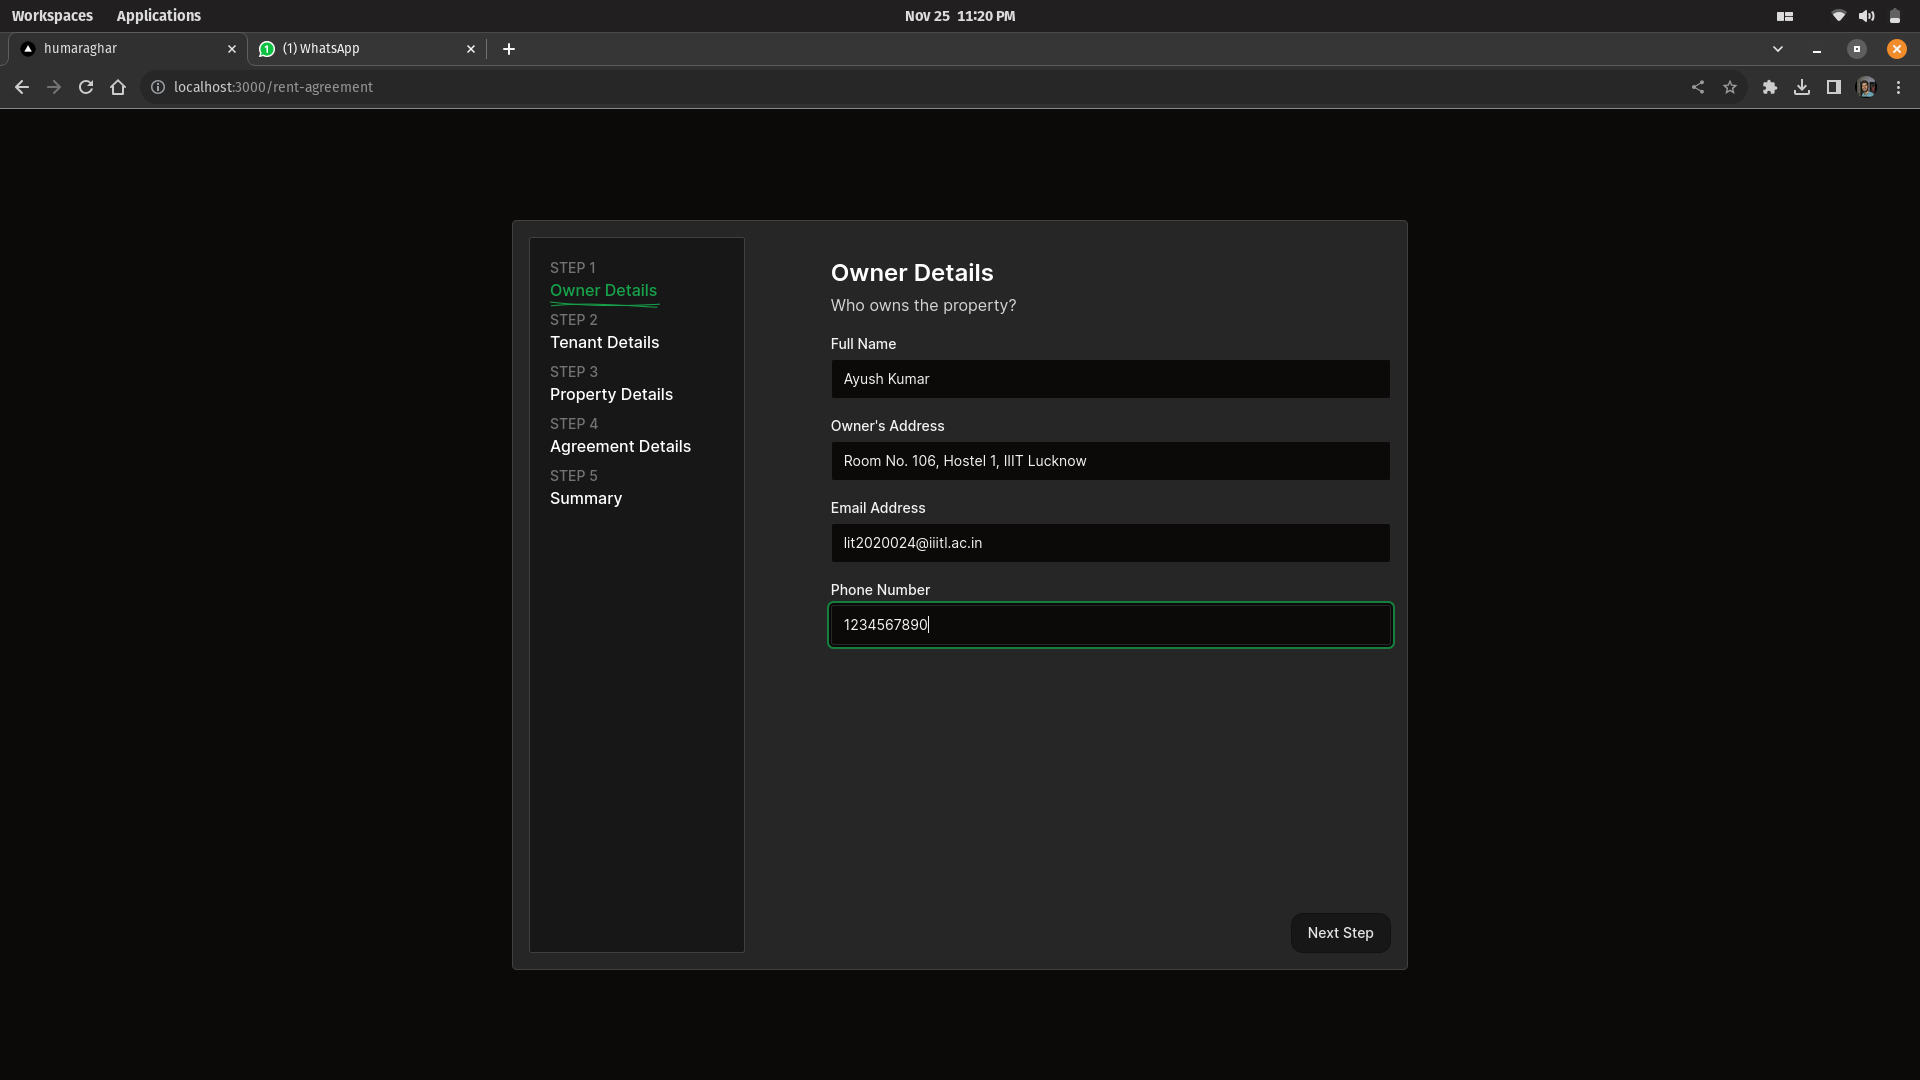
\includegraphics[width=0.8\textwidth]{Images/screenshots/agreementform.png}
        \caption{Rent Agreement Form}
    \end{figure}

    \begin{figure}[h]
        \centering
        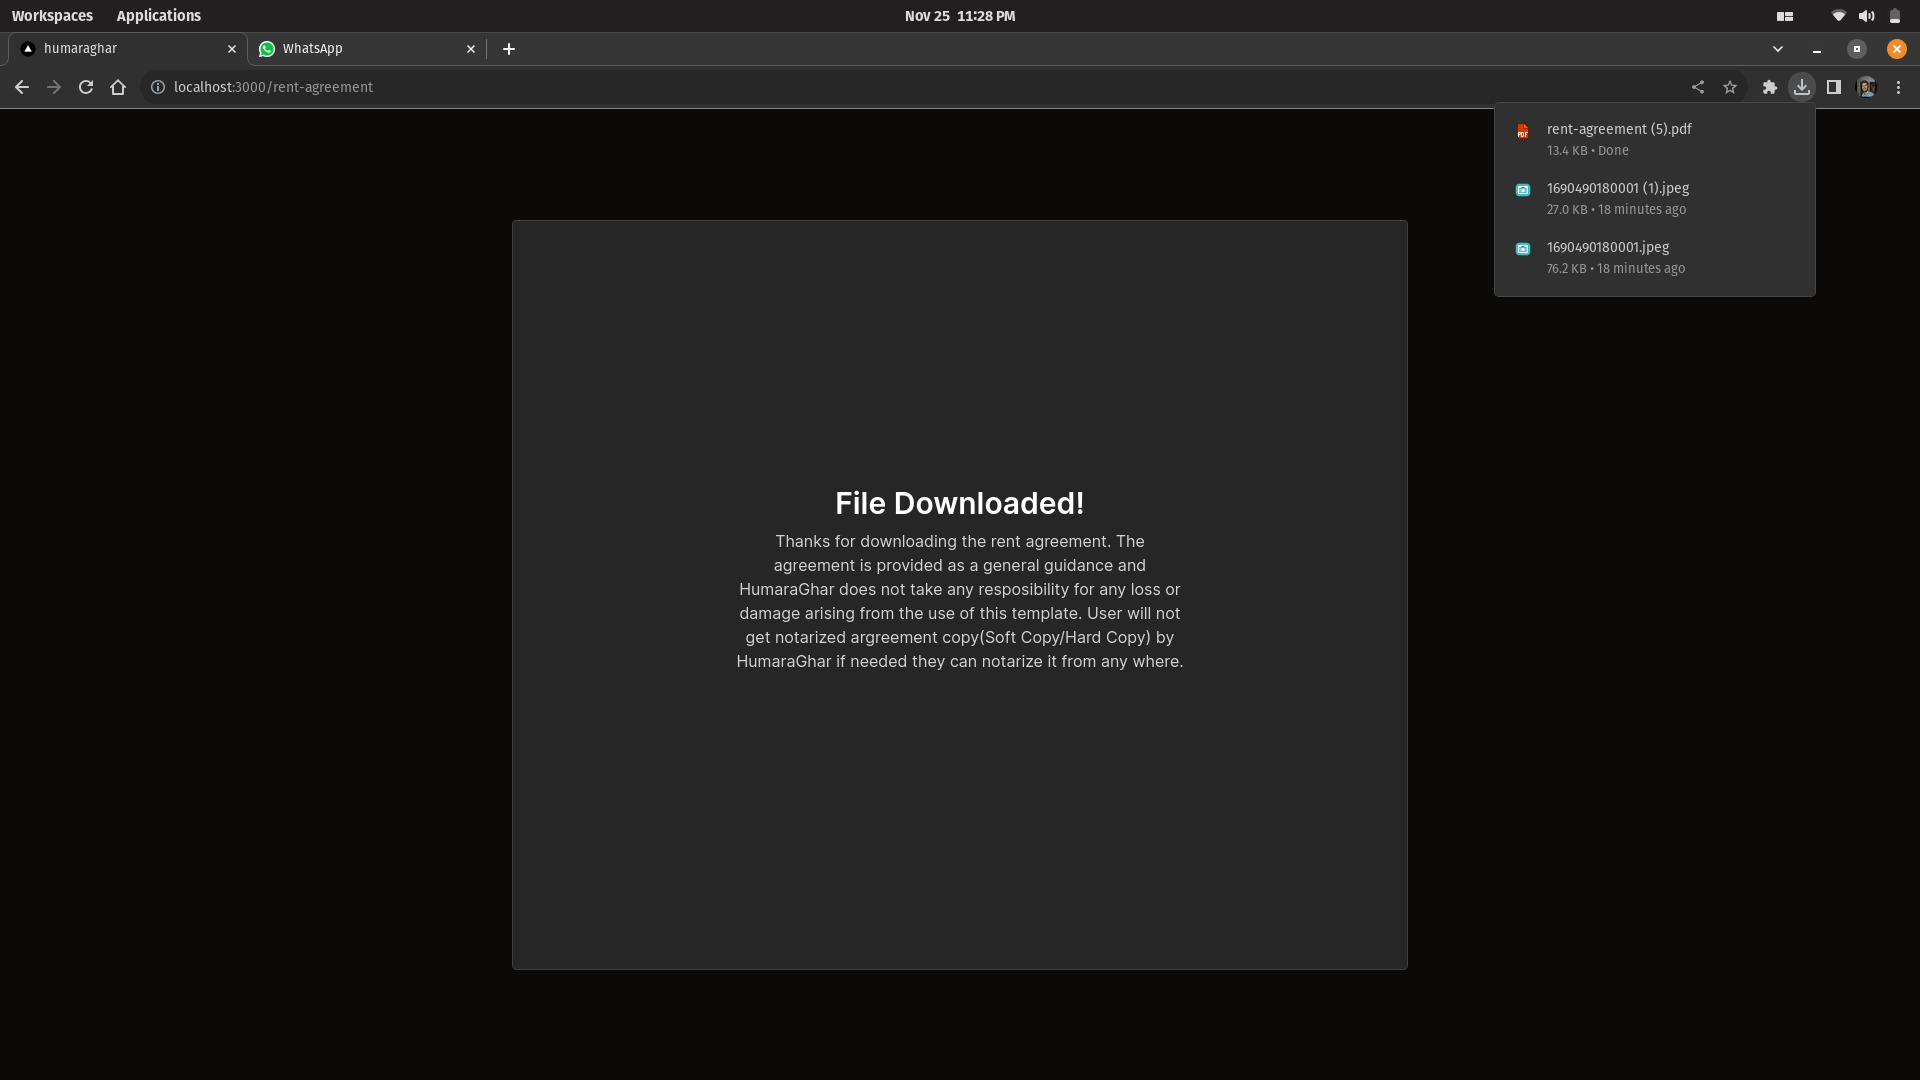
\includegraphics[width=0.8\textwidth]{Images/screenshots/agreementdownload.png}
        \caption{Rent Agreement Download}
    \end{figure}

}

\par\bigskip\bigskip
\subsection{Admin Panel}
To stop spam property listings, especially for non-shared rooms, they have to go through a manual acceptance before they are shown to the public.
Currently only the project owners have admin access. The admin panel is used to view all the pending listings and accept or reject them.

\begin{figure}[h]
    \centering
    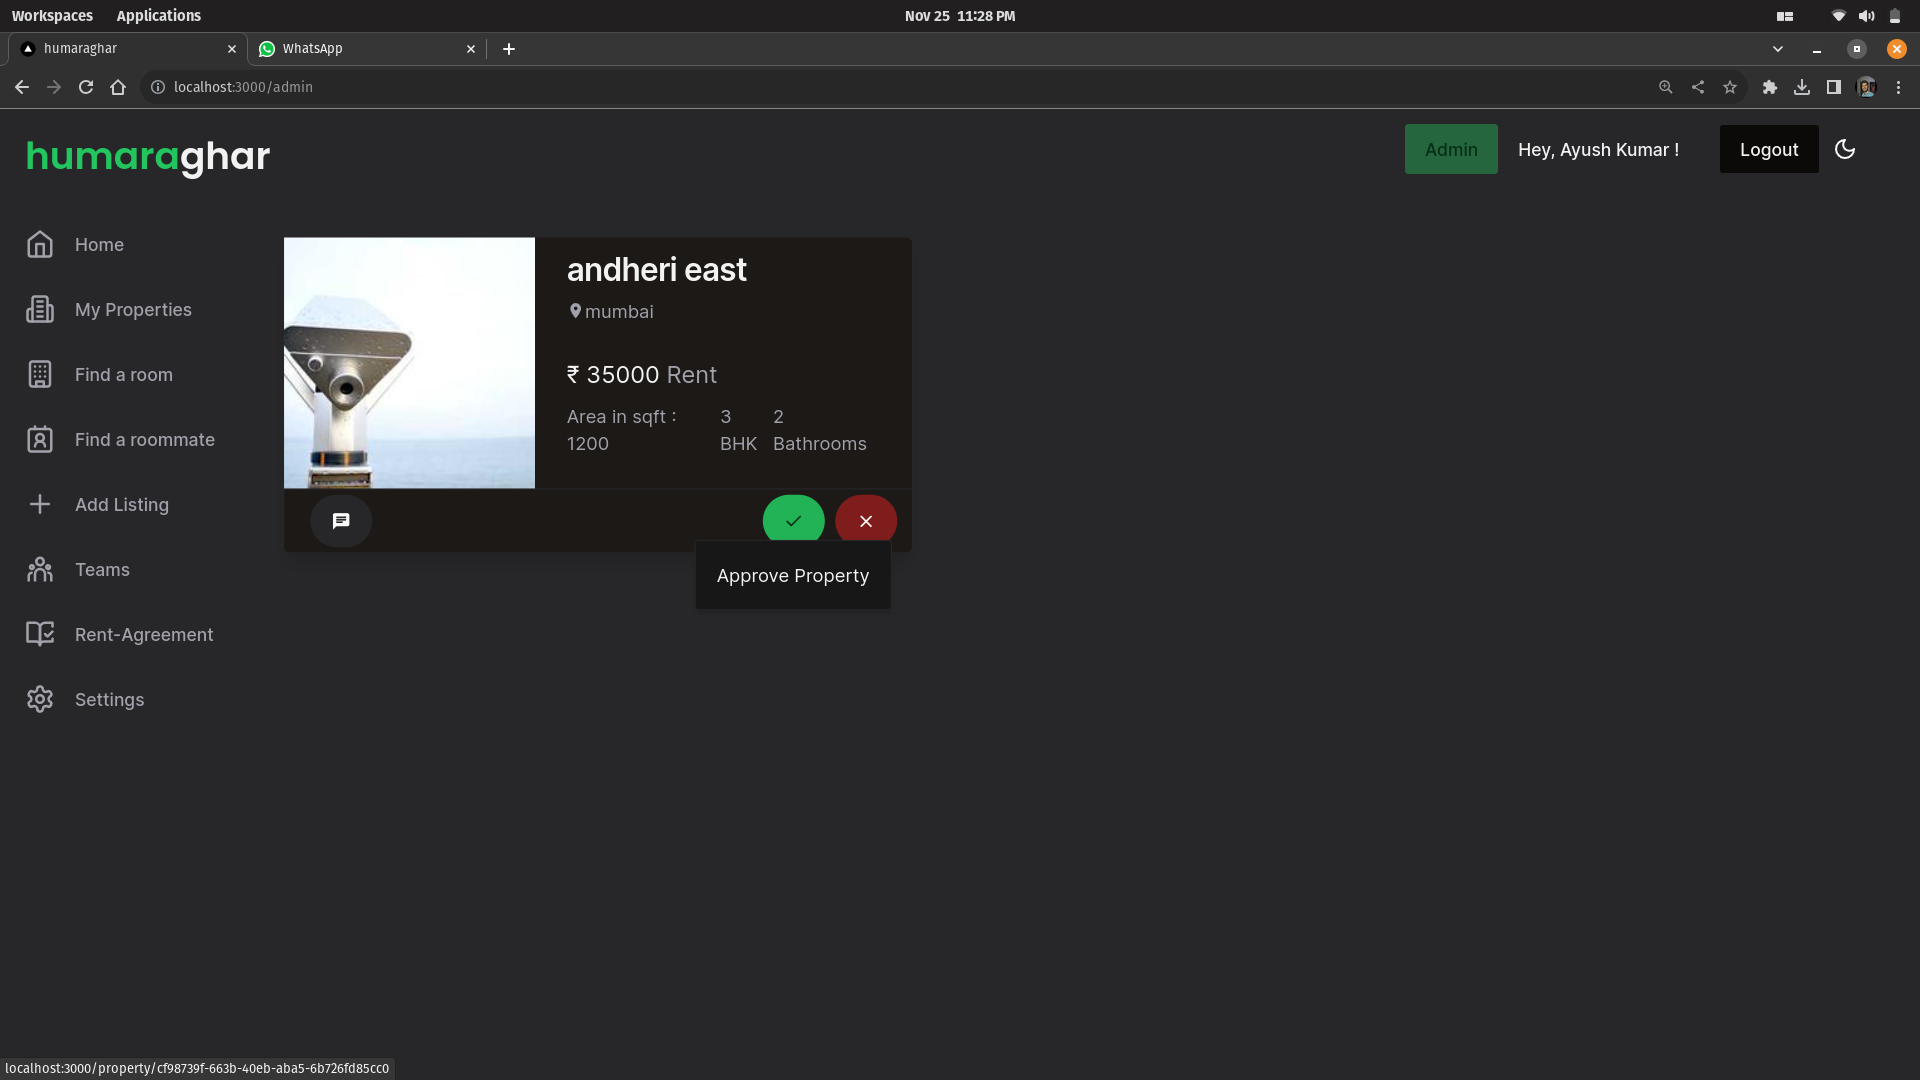
\includegraphics[width=0.8\textwidth]{Images/screenshots/admin.png}
    \caption{Admin Panel}
\end{figure}